\documentclass[a4paper,10pt]{article}
\usepackage[utf8]{inputenc}
\usepackage{amsmath}
\usepackage{graphicx}
\usepackage{subcaption}
\usepackage[font=footnotesize]{caption}
\usepackage{hyperref}
\usepackage{float}
\usepackage{epstopdf} 		%Convert EPS files to PDF format
\usepackage{pdfpages} 		%Utility to include pdf documents into the report, used to include datasheets in appendices.
\usepackage{tikz} 			%Utility to draw nice figures
\usepackage{circuitikz} 	%Utility to draw circuits in tikz

\usepackage{chngcntr}
\counterwithin{figure}{section}
\counterwithin{equation}{section}

\usetikzlibrary{shapes, arrows, chains, scopes, positioning}

\tikzstyle{block} = [draw, fill=blue!20, rectangle, minimum height=3em, minimum width=6em]
\tikzstyle{blockg} = [draw, fill=green!20, rectangle, minimum height=3em, minimum width=6em]

\usepackage{todonotes}
\usepackage{listings}
\usepackage{dcolumn}

\usepackage{fullpage}

\usepackage{xcolor}
\hypersetup{
    colorlinks,
    linkcolor={red!50!black},
    citecolor={blue!50!black},
    urlcolor={blue!80!black}
}

\setlength{\parindent}{0pt}

\title{Drives and Control - DC Motor Speed Control}
\author{Thomas Søndergaard Christensen, Erlingur Ívar Jóhannsson, Mikkel Skarup Jaedicke, Catalin Ionut Ntemkas}
\date{dd/mm/yyyy}


\begin{document}


\begin{titlepage}
\begin{center}

\textsc{\LARGE University of Southern Denmark}\\[1.5cm]
\textsc{\Large MSc in Engineering - Electronics}\\
\textsc{\large Drives and Control}\\[0.5cm]
\vfill
\hrule ~\\[0.3cm]
{ \huge \bfseries DC Motor Speed Control\\[0.4cm] }
\hrule ~\\[1.5cm]
\vfill

% Author and supervisor
\begin{minipage}[t]{.49\textwidth}
\begin{flushleft} \large
\textbf{Author:}\\
ddmmyy Catalin\\
ddmmyy Mikkel Skarup Jaedicke\\
ddmmyy Erlingur Ívar Jóhannsson\\
100589 Thomas S. Christensen
\end{flushleft}
\end{minipage}
\begin{minipage}[t]{.49\textwidth}
\begin{flushright} \large
\textbf{Supervisors:} \\
Jacob Lykke Pedersen\\
\end{flushright}
\end{minipage}

\vspace{1.2cm}
Date: 11-04-2016

\end{center}
\end{titlepage}


\newpage
\tableofcontents
\newpage
\listoffigures
\listoftables
\listoftodos
\clearpage
\newpage
%!TEX root = ../main.tex
\section{Introduction}
\todo[inline]{Do something about list of figures - Mikkel}

Designing a control system for a DC motor is a multi-step process. It involves the parametrization of the system, the design of the controller as well as simulations and experiments to determine what is the best strategy to follow in certain situations depending on the plant. The purpose of this DC report is to go through these steps and provide the reader with the information required in such a procedure. Also, this report has been written using the citation~\cite{feedback} as the main source of theoretical knowledge. The motor models that are used are the Pittman 9234S007-R1 and 9234S006~\cite{pittmann}.
\\

Finding the parameters such as the inductance and the constants of a motor can be achieved by experimental procedures in a laboratory environment using the appropriate instruments. The parameters that required to be calculated are the voltage constant, the armature resistance, the viscous damping factor and the motor inductance and inertia. In many cases, more than one experiment are done as well as more than one methods are followed for greater accuracy of the data. Then, the data is compared with the datasheet of the motors to see if the values coincide or if they deviate. The parameters found by the experiments are used as input to different controllers to drive and test the motor. 
\\

Designing a controller requires analysis of different topologies such as the PID and IPD as well as the required order needed to control the motor effectively. Also, their transfer functions need to be analysed and comprehended in order to better understand how they function. Apart from that, implementing different strategies to improve the behaviour of the overall system such as noise filtering and anti-windup design plays an important role in the process of designing a controller. The effectiveness of these strategies are not only affected by the environment and the overall system, but also from the settling time, which is a very important variable to take into account. Lastly, the parameters are inserted in the gain equations of the controllers to receive the gains for a specified system.
\\

After designing a controller, simulations must be run in order to examine how the system is expected to behave in various circumstances and under ideal conditions. Different controllers are being examined so the most efficient and suitable one can be chosen for a specific purpose. Specifically, the IPD and PI are tested under this report with and without load or extra inertia at different speeds. The two controllers are also tested under real conditions using the Pittman motors with the same parameters such as speed and load step that are used under the simulations. Finally, the results from the real world and the simulated experiments are compared to each other to observe any similarities or differences at the overall system's behaviour.

\todo{make the sections go to the next page)}
\todo{fix the pages, there are some spaces towards the end. Large spaces!}
\newpage
%!TEX root = ../main.tex
\section{Hardware implementation}
The group was given 2 Pittman 9234 24V motors,\todo{Mikkel, check this change. I added the models of the motors.} the models being 9234S007-R1 and 9234S006, a dual H-bridge and a dSPACE system.
One of the Pittman motors was equipped with a rotational encoder.
The dSPACE system is connected to the H-bridge which drives the motors. 
The setup can be seen in figure~\ref{fig:implementation_block}.
Furthermore the encoders of the motor is connected to the dSPACE system.
A Lecroy wavesurfer 2054 oscilloscope with current probes and KE 34310A multimeters are used in the various experiments.

\begin{figure}[!h]
\centering
%!TEX root = ../main.tex

%\documentclass{standalone}

%\usepackage{tikz}

% The block diagram code is probably more verbose than necessary
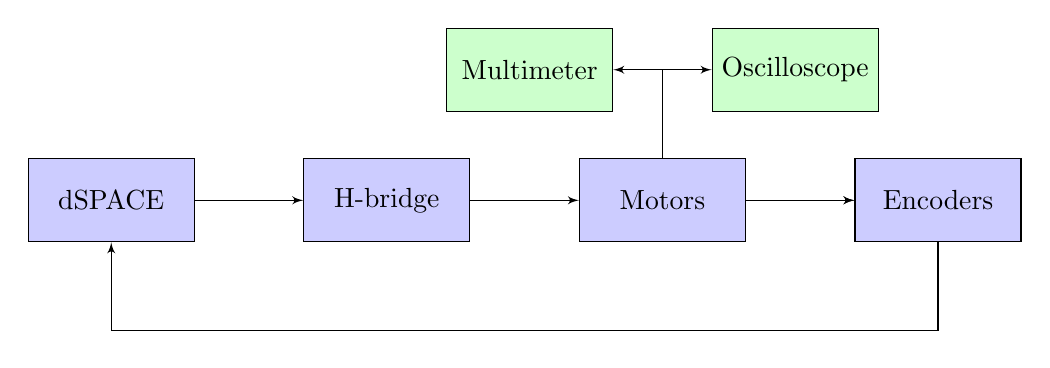
\begin{tikzpicture}[auto, node distance=3.5cm,>=latex']
    % We start by placing the blocks
    \node [block] (motor) {Motors};
    \node [block, left of=motor] (hbro) {H-bridge};
    \node [block, left of=hbro] (dspace) {dSPACE};
    \node [block, right of=motor] (encoder) {Encoders};
    \node [below= 1cm of motor] (point) {};
    \node [above= 1cm of motor] (point1) {};
    \node [blockg, right =0.5cm of point1] (scope) {Oscilloscope};
    \node [blockg, left =0.5cm of point1] (multi) {Multimeter};


    \draw[->] (hbro) -- (motor);
    \draw[->] (dspace) -- (hbro);
    \draw[->] (motor) -- (encoder);
    \draw[->] (motor) -- (encoder);
    \draw[-] (encoder) |- (point.west);
    \draw[->] (point) -| (dspace);
    \draw[->] (motor) |- (scope);
    \draw[->] (motor) |- (multi);


  %\node[label=above:C] (C)  [below right=0.7cm and 4cm of B1]
   %    {($2m-1$)};
    %\draw [draw,->] (input) -- node {$r$} (sum);
    %\draw [->] (sum) -- node {$e$} (controller);
    %\draw [->] (system) -- node [name=y] {$y$}(output);
    %\draw [->] (y) |- (measurements);
\end{tikzpicture}

%\end{document}


  \caption{Block diagram showing the motor setup.}
  \label{fig:implementation_block}
\end{figure}


\newpage
%!TEX root = ../main.tex
\section{Modelling a DC motor}
This section deals with the modelling and parametrization of a brushed DC motor, specifically the Pittman 9234S007-R1 24V servomotor.
Figure \ref{fig:dcmotormodel} is a simple model of a DC motor.
The parameters of this model will be estimated by experimentation.
\todo[inline]{Is this really a servo motor? - Mikkel}
\todo[inline]{Maybe the viscous friction should be Kv here? - Mikkel}


\begin{figure}[!h]
	\centering
	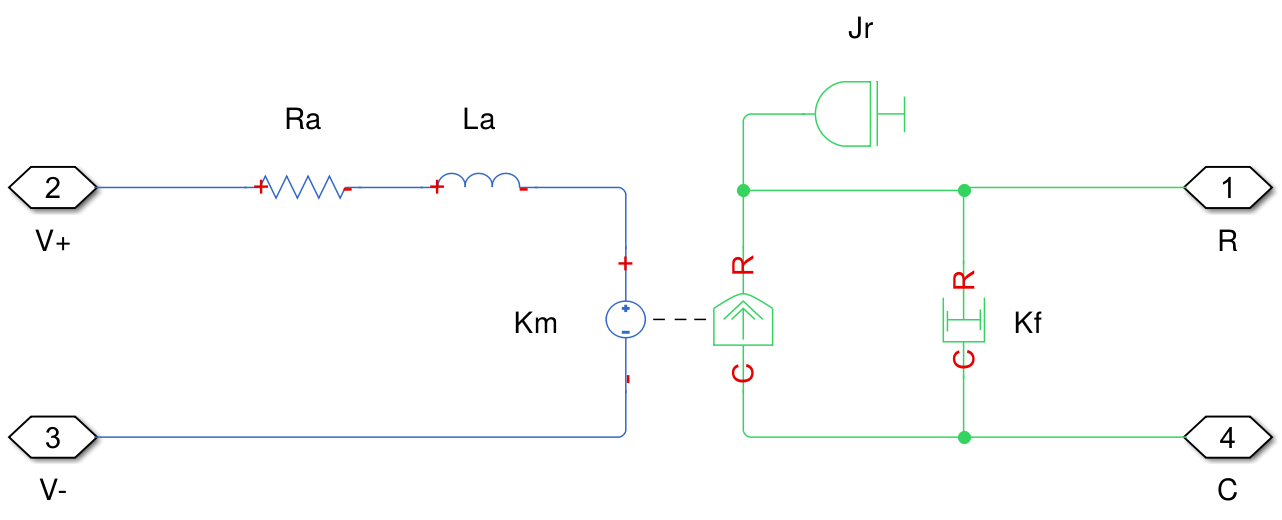
\includegraphics[width=.75\linewidth]{graphics/dcmotormodel.png}
	\caption{Simulink model of a brushed DC motor.}
	\label{fig:dcmotormodel}
\end{figure}

For the experiments a test setup is supplied. 
A diagram of the setup can be seen in figure~\ref{fig:motorsetup}. 
As the figure shows, two motors are connected by the shafts through an external inertia.
The shafts of the two motors will rotate in opposite directions given the same voltage.
To simulate this, a gearbox (called Inverter on the figure) with gear ratio -1:1 is placed between the two motors.
Finally, the Pittman 9234S007-R1 is equipped with an encoder to be used for monitoring of the angular velocity of the shaft.


\begin{figure}[!h]
	\centering
	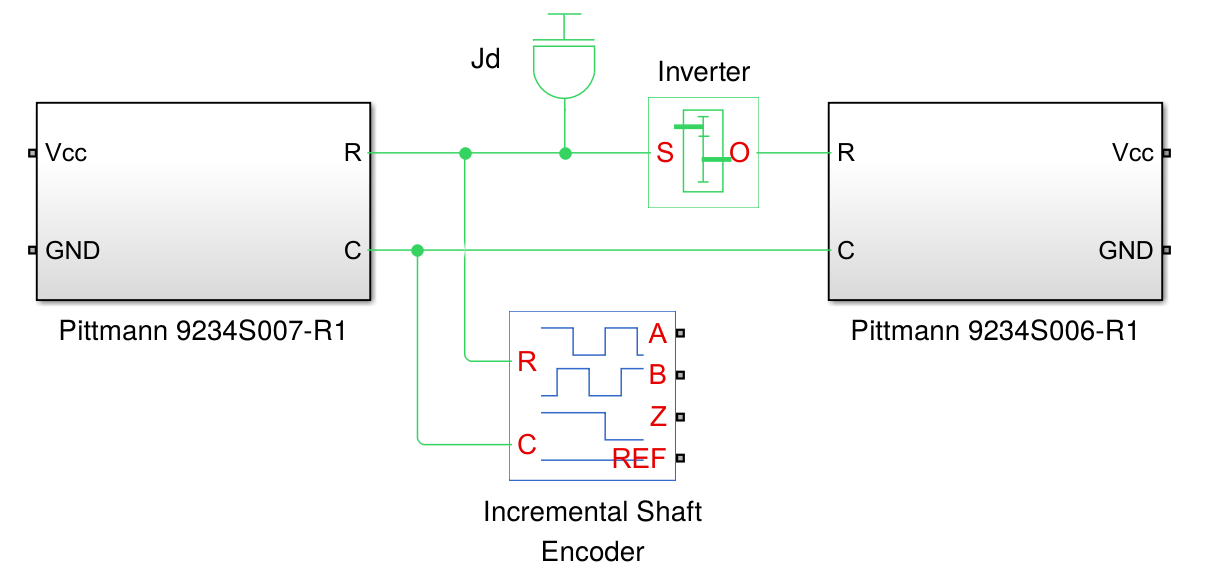
\includegraphics[width=.8\linewidth]{graphics/motorsetup.png}
	\caption{Simulink model of the motor setup provided for the project.}
	\label{fig:motorsetup}
\end{figure}

\subsection{Voltage Constant - $K_e$}
\label{sec:voltconstat}
The voltage constant describes the relationship between angular velocity of the rotor and the resulting back-EMF:
\begin{equation}
	\label{eq:voltconstant}
	K_e\omega_r = V_{bmf}
\end{equation}
where $\omega_r$ is the angular velocity of the rotor and $V_{bmf}$ is the back-EMF across the motor.
From equation~\ref{eq:voltconstant} it is apparent that $K_e$ can be determined if the voltage across the terminals of the motor is measured while the motor is being run at a known velocity.
The experiment is conducted as follows:
A voltage is applied across the terminals of the Pittman 9234S006.
The resulting velocity of the assembly is monitored using the encoder on the Pittman 9234S007-R1.
Across the terminals of this motor is now only the back-EMF value, which is recorded.
Figure~\ref{fig:velvsvolt} shows the recorded data. 
As is expected, there is a highly linear relationship between the voltage and velocity.
The final value of $K_e$ is determined by averaging and then dividing the collected data.
$$K_e=\frac{V_{bmf}}{\omega_r}=0.0360$$
This value is within 1.2\% of the value given in the datasheet~\cite{pittmann}.

\begin{figure}[!h]
	\centering
	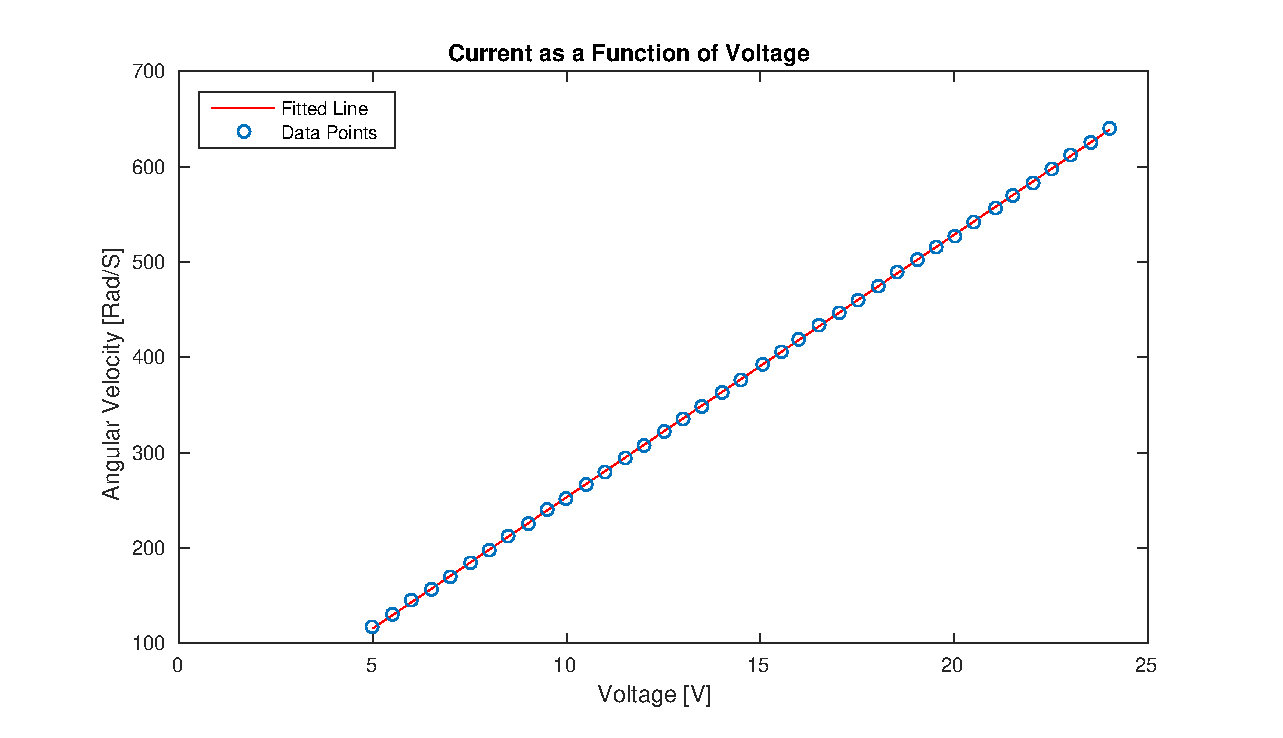
\includegraphics[width=.75\linewidth]{graphics/vvsrpm}
	\caption{Angular velocity of the shaft at different voltages.}
	\label{fig:velvsvolt}
\end{figure}

\subsection{Armature Resistance - $R_a$}
\label{sec:armature}
\paragraph{Method I}~\\
The armature resistance, $R_a$ in figure~\ref{fig:dcmotormodel}, can simply be found by applying Ohm's law.
The current through a resistor is well defined when a voltage is applied across it.

\begin{figure}[!h]
	\centering
	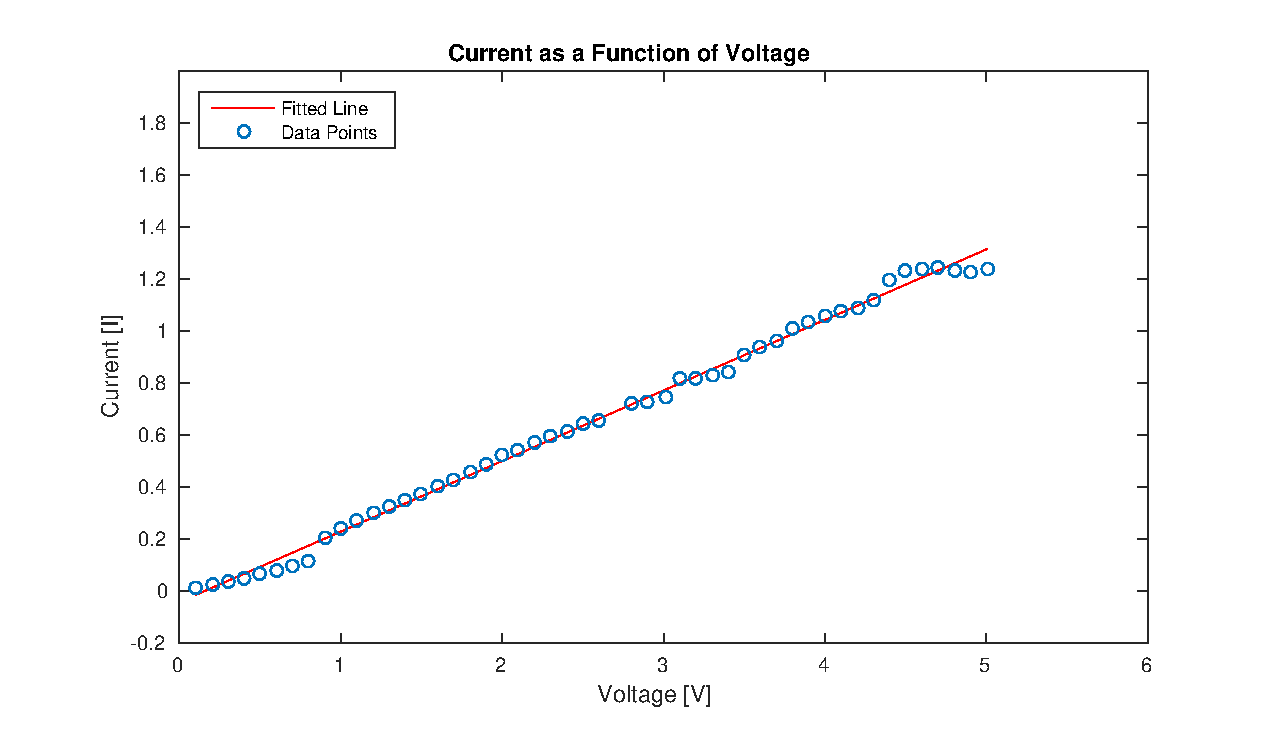
\includegraphics[width=.75\linewidth]{graphics/raplot}
	\caption{Current as a function of voltage with the rotor blocked.}
	\label{fig:raplot}
\end{figure}

However, when the rotor is spinning, the circuit produces back-EMF.
This counters\todo{by saying counters, do you mean counteracts?} the input voltage, effectively lowering the current through $R_a$.
In order to avoid this effect the rotor is blocked.
Since with a blocked rotor there will be no change in voltage in the system, the inductor acts as a short circuit, reducing the circuit to a voltage across a resistor. 

Figure~\ref{fig:raplot} shows the data collected in order to determine the value of the armature resistance.
A voltage is applied across the terminals at 0.5 V.
According to the datasheet~\cite{pittmann} the current at maximum allowed continuous torque is 1.75 A.
This current is reached at 5 V, therefore, the measurements stop there.
As it can be seen from the figure, a line is fitted to the data.
This is done using the linear least squares method with the following result:
$$I(V)=0.274\cdot V-0.047$$
with $R^2=0.996$.
Since for the plot $I(V)$:
$$R_a = \frac{1}{\text{slope}} = 3.647\Omega$$

This value is significantly higher, approximately 25\% higher than the value given in the datasheet.
Additionally, the final data points seem to become irregular.
This is likely caused by the high currents drawn by the motor at these voltages warming the motor and therefore slightly altering the characteristics of the resistor.
Additionally, at $I(0)$ this model will result in a small negative current.
Obviously, this is not correct; no current would be expected at zero voltage.
Adjusting the model such that it will intersect the origin results in a higher resistance of $R_a=3.888\Omega$.

For these reasons it has been decided to pursue different means of determining the armature resistance:
\paragraph{Method II}~\\
This method makes use of the voltage constant found in section~\ref{sec:voltconstat}.
By expanding $V_{cc}$ in equation~\ref{eq:voltconstant} an expression for $R_a$ can be found:
\begin{equation}
	\label{eq:voltconstantexpanded}
	K_e\omega_r = V_{cc} = I_aR_a\quad \Rightarrow \quad R_a = \frac{\omega_rK_e}{I_a}
\end{equation}
Similarly to the experiment in section \ref{sec:voltconstat}, one motor is used to spin the other to speed.
This time, however, the terminals of the Pittman 9234S007-R1 are connected through a power resistor, $R_e$.
Obviously then:

\begin{eqnarray}
	R_t =& R_a + R_e\\
	R_a =& \frac{\omega_rK_e}{I_a}-R_e
\end{eqnarray}

where $R_t$ is the total resistance in the system.
As the voltage across the terminals of the Pittman 9234S006 is increased the resulting velocity and current are noted.
Finally, the armature resistance is found to be:
$$R_a = 3.715\Omega$$

This value, curiously, coincides with the one found using method I.

\subsection{Viscous Damping Factor - $K_v$}
\label{sec:viscous}
At steady state with no load the torque generated by the motor must be exactly equal to the friction present in the system.
Generally, three types of friction are expected in a DC motor: viscous friction ($T_v$), coulomb friction ($T_c$) and static friction ($T_s$).
Figure~\ref{fig:friction} is a depiction of their interaction.
Formally:
\begin{equation}
	\label{eq:totfriction}
	T_e-(T_s+T_c+T_v)=0
\end{equation}
Viscous friction is proportional to the angular velocity, $\omega_r$ by the factor $K_v$.
Determining this factor is the goal of this section.
Since $T_v=K_v\omega_r$ and $T_s$ are negligible at high values of $\omega_r$ equation~\ref{eq:totfriction} can be rewritten as:
\begin{equation}
	\label{eq:frictionnostatic}
	T_e-(T_c+K_v\omega_r)=0 \quad \Rightarrow \quad K_v = \frac{T_e-T_c}{\omega_r}
\end{equation}

$T_e$ can be determined from the torque constant, $K_t$, which, in the case of the DC motor is equal to $K_e$ such that:
$$K_e = \frac{T_e}{I_{ss}} \quad \Rightarrow \quad T_e = K_eI_{ss}$$

\begin{figure}[!h]
	\centering
	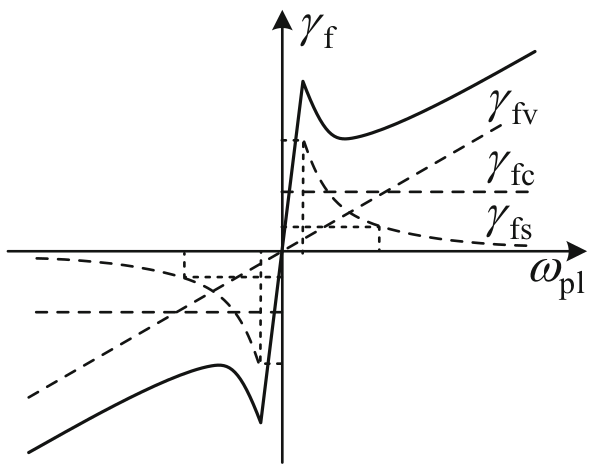
\includegraphics[width=.5\linewidth]{graphics/friction}
	\caption[The three friction components]{The three friction components: viscous, coulomb and static.}
	\label{fig:friction}
\end{figure}

Where $I_{ss}$ is the current through the motor at steady state.
Figure~\ref{fig:tqangle} shows $T_e$ as a function of $\omega_r$.
As it can be seen, the relationship is mostly linear when $\omega_r>300\frac{Rad}{S}$.
Fitting a line to the linear part of this graph can be used to determine $T_c$.
This line will have the same slope as $K_v$ and will therefore cross the y-axis at $T_c$.

\subsubsection{Experiment}
This experiment is conducted during no-load condition on the Pittman 9234S007-R1, as velocity measurements are required.
Initially, a voltage ranging from 0-24 V in 0.5 V steps was applied to the terminals of the motor. However, in order to better capture the effects of $T_s$, the range 0-1 V was recorded using 50 mV steps and from 1-2 V using 100 mV steps.
During each step the current through the motor and angular velocity of the rotor are recorded.
Using the value of $K_e$ found in section~\ref{sec:voltconstat} it is possible to calculate $T_e$, see figure~\ref{fig:tqangle}. The fitted line seen on figure~\ref{fig:tqanglefull} is found to intersect the y-axis at:
$$T_c=0.0028$$
\begin{figure}[!h]
	\begin{subfigure}[t]{.49\linewidth}
		\centering
		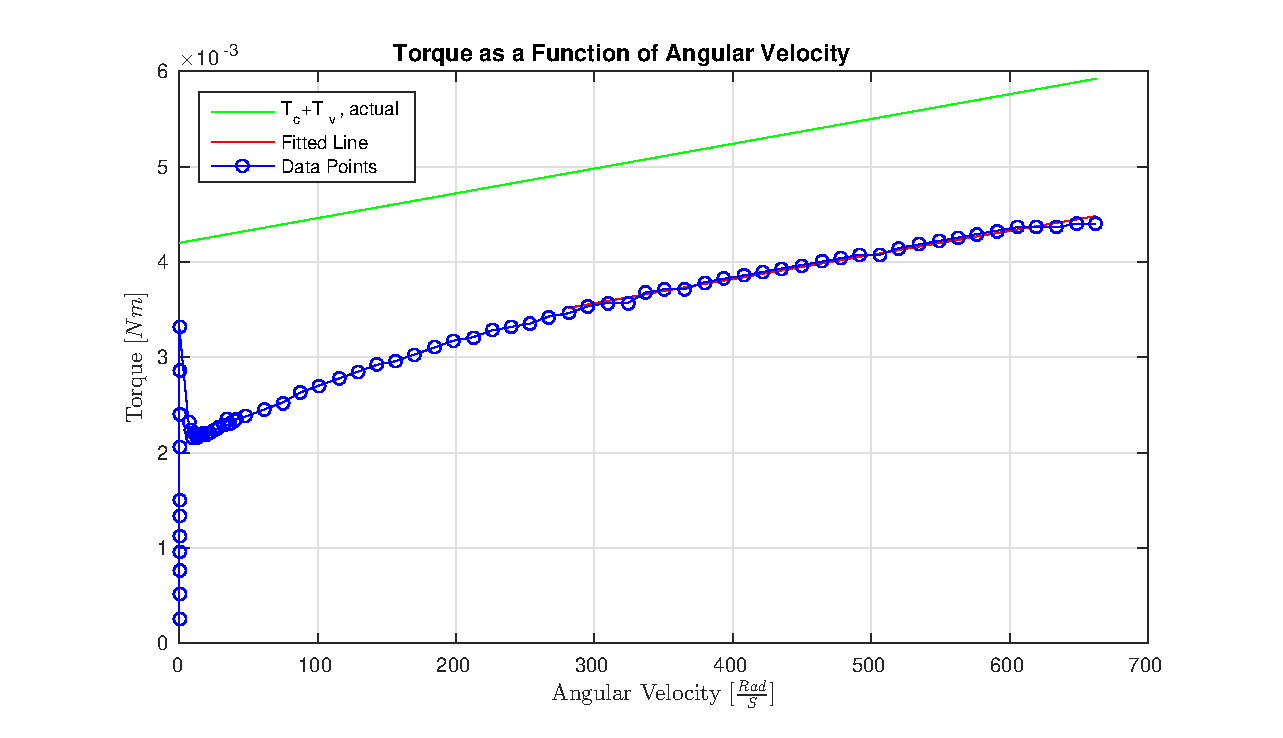
\includegraphics[width=\textwidth]{graphics/tevel}
		\caption{Full range, 0-24V.}
		\label{fig:tqanglefull}
	\end{subfigure}
	\begin{subfigure}[t]{.49\linewidth}
		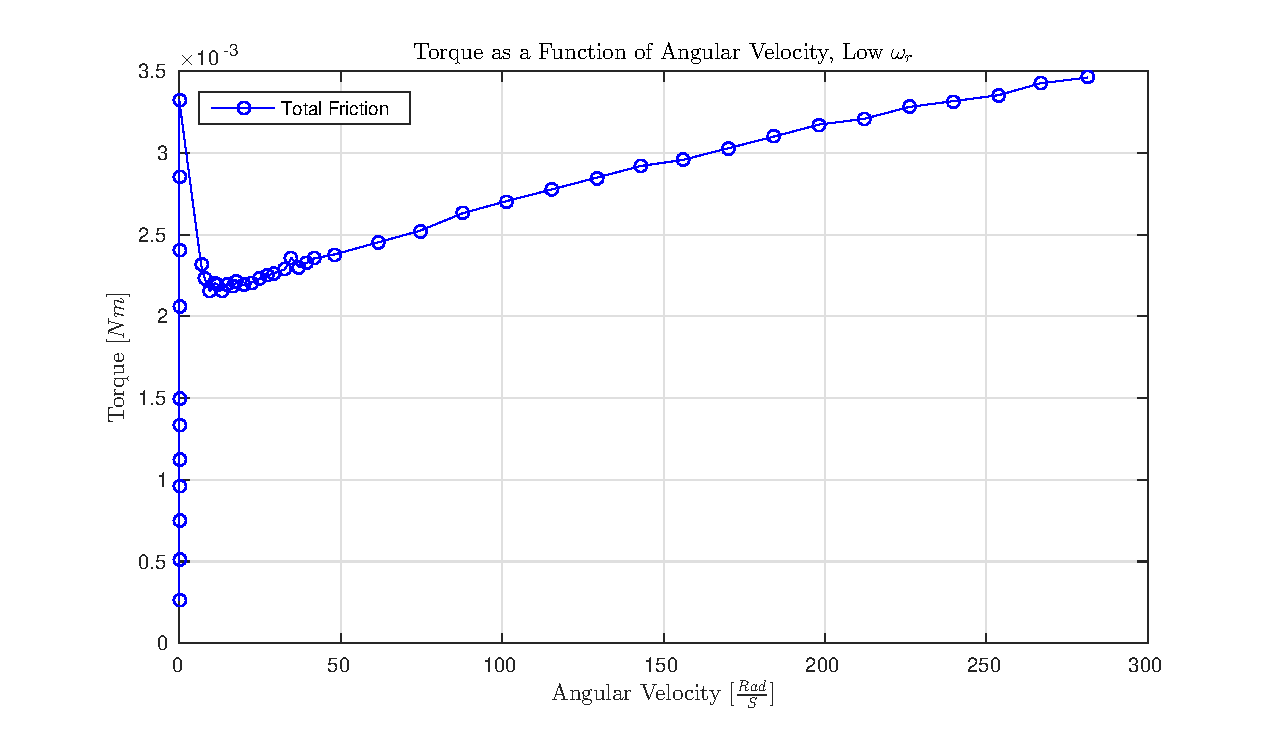
\includegraphics[width=\textwidth]{graphics/tevel_low}
		\caption{Partial range, 0-5V}
		\label{fig:tqanglelow}
	\end{subfigure}
	\caption[Torque as a function of angular velocity]{Torque as a function of angular velocity. The fitted line represents the linear part of the total friction. The green line shows the value according to the datasheet.}
	\label{fig:tqangle}
\end{figure}

Applying this value allows the calculation of $K_v$, see figure~\ref{fig:visvel}.
Ideally, as $\omega_r\rightarrow \infty$ this graph will converge to the value $K_v$. 
Similarly to figure~\ref{fig:tqangle}, at low values of $\omega_r$, $T_s$ is significant and therefore is not negligible.
For this reason the value $K_v$ is taken as the average of every reading where $\omega_r>300\frac{Rad}{S}$. 
This is the point where, by inspection, $T_e$ is mostly linear with increasing $\omega_r$:
$$K_v=2.611\cdot 10^{-6}$$
Additionally, figure~\ref{fig:tqanglelow} shows the initial effect of the static friction on the system.
The highest recorded static friction is $T_s=3.327*10^{-7}$.
\begin{figure}[!h]
	\centering
	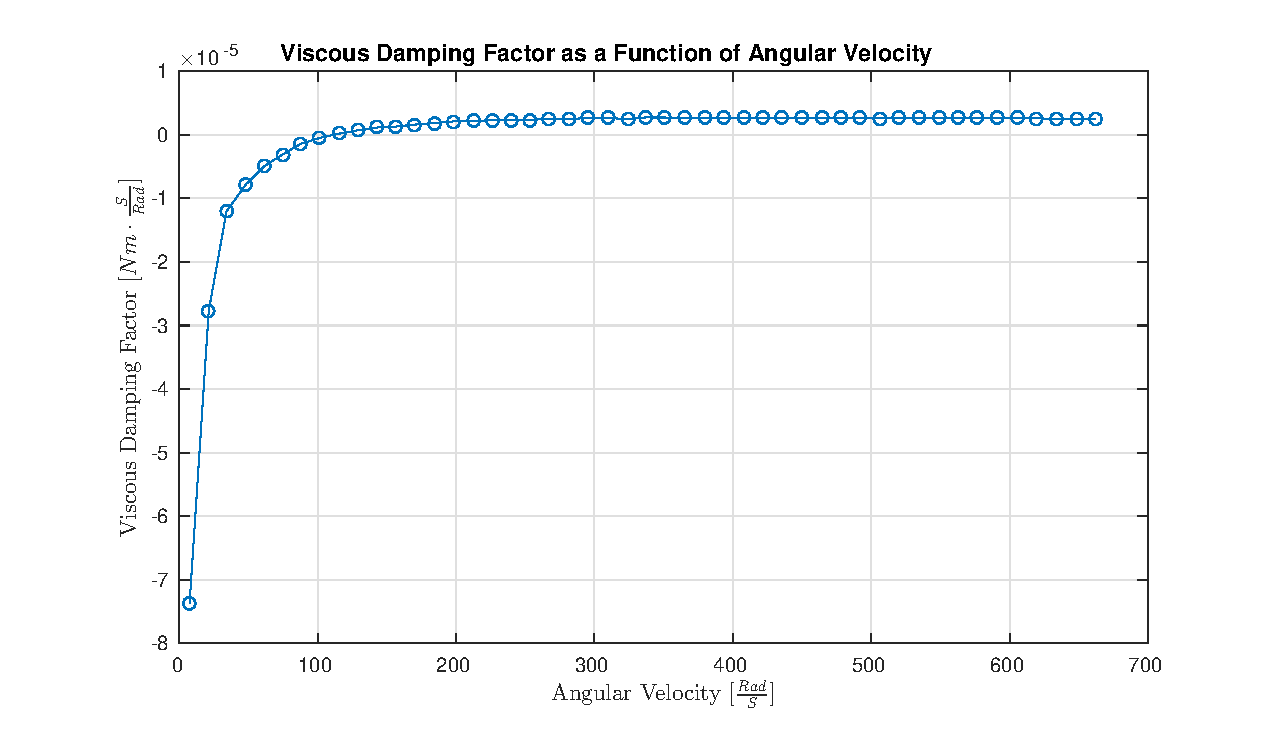
\includegraphics[width=.75\linewidth]{graphics/visvel}
	\caption{Viscous damping factor as a function of angular velocity.}
	\label{fig:visvel}
\end{figure}
\subsubsection{Discussion}
The value of the viscous damping factor $K_v$ found, is within 1.0\% of the value given in the datasheet, which is a satisfactory result.
Looking at the coulomb friction found using this method however, reveals a value that is significantly smaller, 0.0028, than the one listed in the datasheet, 0.0042.
This can be seen in figure~\ref{fig:tqangle}. 
The green line in the figure shows the value of $T_e$ given the values of $K_v$ and $T_c$ of the datasheet.
As it can be seen, the slope, and therefore the values of $K_v$ are nearly identical.
A reasonable explanation for this inconsistency has yet to be devised.

\subsection{Motor inductance - $L_a$}
\label{sec:incuctance}
\paragraph{Method I}~\\
The inductance of the motor, $L_a$ in figure~\ref{fig:dcmotormodel}, can be found by looking at the transient response of the stalled motor. 
When the motor is stalled there is no back-EMF in the circuit. The motor can then be modelled as a simple RL-circuit. 
An RL-circuit has a known time constant $\tau$.
$$\tau = \frac{L}{R_{total}}$$
The time constant is defined as the time it takes for the voltage across the component to rise or fall to $\frac{1}{e}$ of the final value.
Measuring the time constant would require measuring the voltage across the inductor or the resistor in the motor. This is not possible as these are built-in. 
Therefore an extra resistor, $R_e$, was put in series with the motor and the voltage across it was measured by an oscilloscope. 
$$\tau = \frac{L}{R_{total}} = \frac{L_a}{R_a+R_e}$$
Rearranging the formula for $\tau$ yields an expression for $L_a$: 
$$L_a = \tau * (R_a + R_e)$$
To give the circuit a step signal it was given a voltage of 8 V by a power supply and then the terminals of the power supply were short circuited by connecting them with a wire thus giving it a step signal with a initial value of 8 V and a final value of 0 V.
The experiment was repeated 10 times. $\tau$ can be found by locating the time where the measured voltage is equal to $\frac{1}{e}$ of the initial voltage.

\subsubsection{Experiment}
The extra resistor, $R_e$, was measured by a multimeter to have a value of $32.97\Omega$.
Then the circuit was given the step signal while measuring the voltage.
The transient responses measured across $R_e$ can be seen in figure~\ref{fig:trans_plot}.

\begin{figure}[!h]
	\centering
	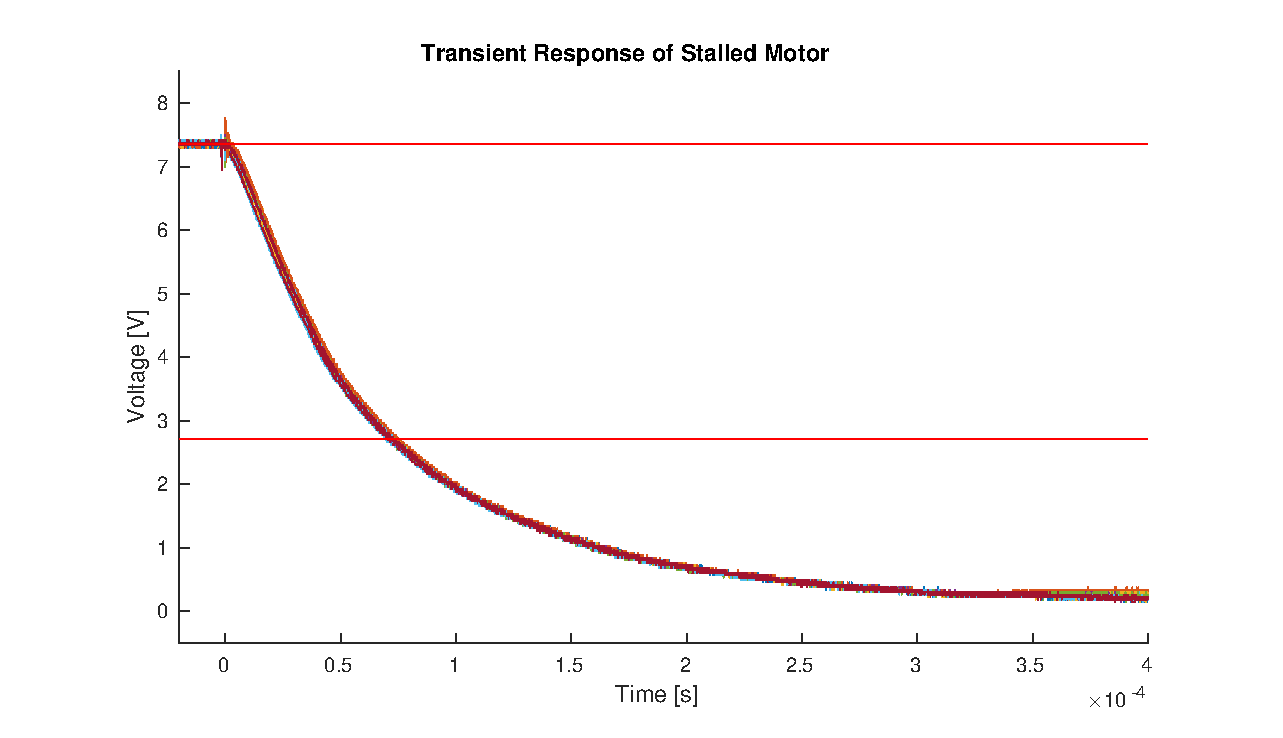
\includegraphics[width=.75\linewidth]{graphics/transient_32ohm}
	\caption{Transient responses measured across $R_e$. The red vertical lines represent the initial voltage, $V_0$, and $\frac{1}{e} \cdot V_0$.}
	\label{fig:trans_plot}
\end{figure}


$\tau$ was found to be 0.713 $\cdot 10^4 s$, by taking the average of the values found from the 10 experiments.
The average value of $L_a$ was then found to be 2.6 mH. The value is only $3.83\%$ higher than the value in the datasheet.

\subsubsection{Discussion}
Only the voltage across $R_e$ is measured, which is problematic as it is assumed in the formula that the transient response is measured across the whole resistance of the circuit. Choosing a value for $R_e$ that is much larger than $R_a$ would minimize the problem.
The experiment was done with values of $R_e$ ranging from $33\Omega$ to $3.3K\Omega$.
Results generally showed that higher values of $R_e$ yielded more difference between the calculated values of $L_a$ and the value given in the datasheet.	
The answer to why this is the case has not been found.


\paragraph{Method II}~\\
The inductance of the motor can be found in another way as shown in this section. 
If the duty cycle $D$ is equal to 0.5 in a dual supply H-bridge the motor will experience the supply voltage positively in one half period and the supply voltage negatively in the next half period.
If the frequency is\todo{Is too low or is NOT too low? Are we sure?} not too low, the motor will not move and no back-EMF is induced in the motor. 
Given that there is no back-EMF the motor can be accurately modelled as an RL-circuit.  
In the first half period the RL-circuit would experience a positive voltage step. 
The voltage step across the inductor will produce a change in current.
This change in current can then be used to calculate the inductance of the motor.
The change in current will produce a change in the voltage across the resistor.
This change in voltage cannot be measured as the resistance is in the inductor, but as long as the current ripple is small the effect is negligible. 
In order to have a small current ripple the frequency cannot be too small.   
The elemental equation for the inductor can easily be rewritten to reveal the inductance when the duty cycle $D$, the voltage $V$, the change in current $\Delta i$ and the time period $T$ are known. 
$$V = L \frac{di}{dt} \Rightarrow \Delta i = \frac{1}{L} \cdot D \cdot T \cdot V $$
$$L = \frac{D \cdot T \cdot V}{\Delta i}$$


\subsubsection{Experiments}
Using dSPACE and a dual supply H-bridge the motor was given a duty cycle of 0.5 at varying frequencies.
A plot of the current and voltage at 30kHz can be seen in figure~\ref{fig:half_duty}.
It can be seen that the voltage change due to the current ripple is negligible as it is not observable.


\begin{figure}[!h]
	\centering
	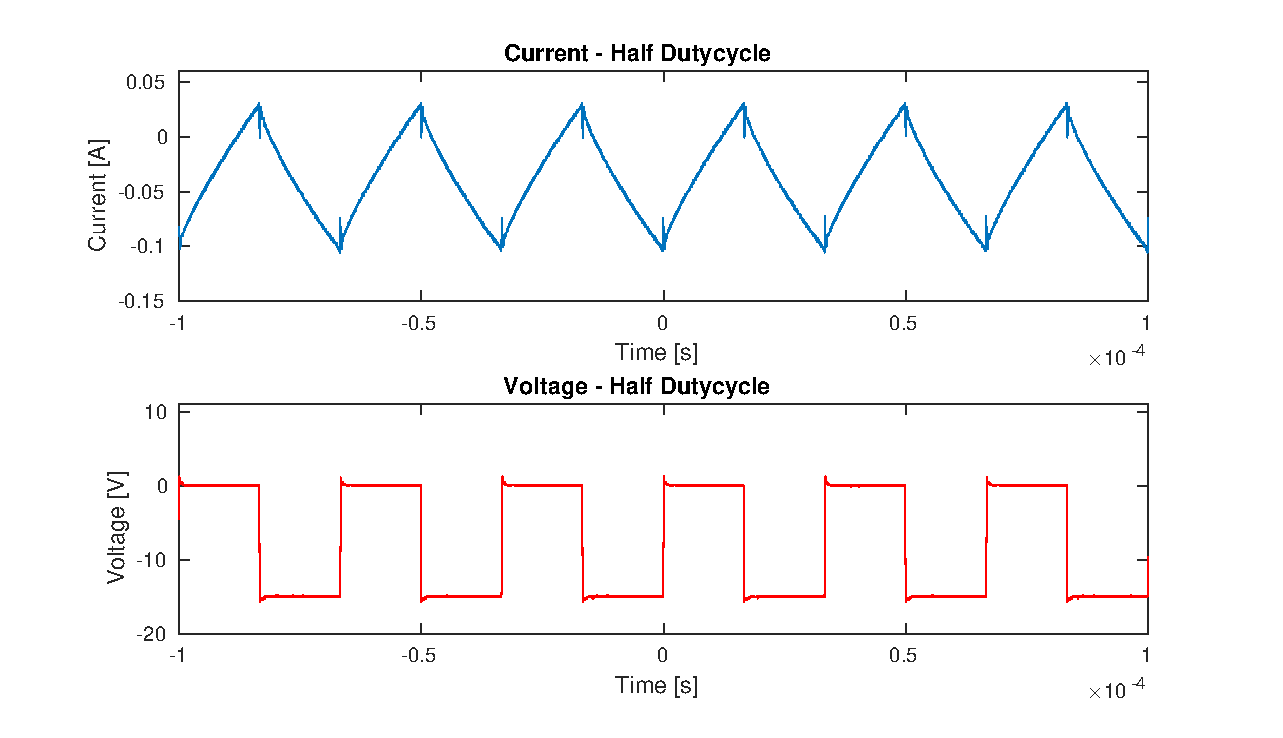
\includegraphics[width=.75\linewidth]{graphics/half_duty}
	\caption{Current and Voltage plots with $D = 0.5$ and a frequency of $30kHz$.}
	\label{fig:half_duty}
\end{figure}

25 experiments were done with frequencies varying from 2kHz to 50kHz.
All data was measured on an oscilloscope and used to calculate the inductance at each frequency.
A plot of the inductance as a function of the frequency can be seen in figure~\ref{fig:inductance_freq}.

\begin{figure}[!h]
	\centering
	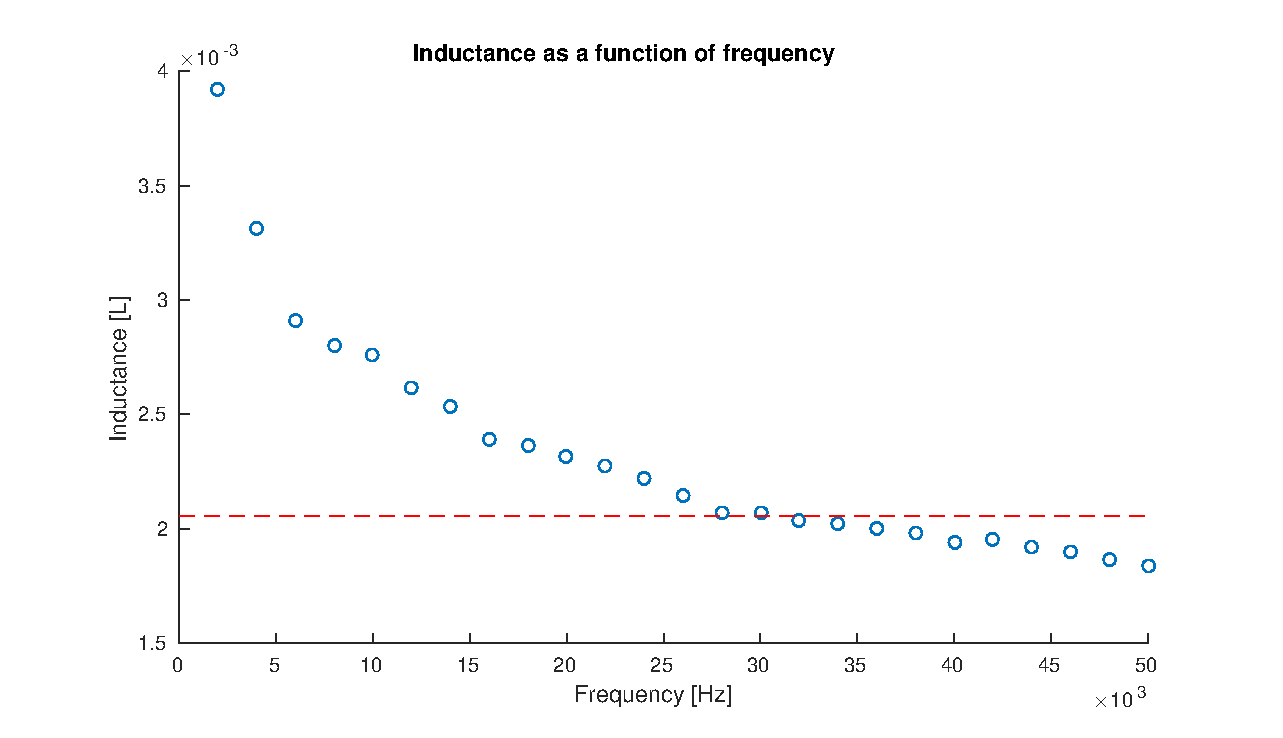
\includegraphics[width=.75\linewidth]{graphics/l_freq}
	\caption{Inductance as a function of frequency. The horizontal line represents the mean value of the inductance measured at frequencies between 25kHz and 35kHz.}
	\label{fig:inductance_freq}
\end{figure}

It can be seen quite easily that the inductance is not a constant, but it is varying with frequency. 
The motor is run at frequencies above 25kHz to be out of the audible range and below 35kHz to avoid too much switching loss. 
Therefore the mean value of all calculated inductances measured between 25kHz and 35kHz is a good approximation of the experienced inductance.
The mean value is found to be 21mH and is shown in figure~\ref{fig:inductance_freq} by a horizontal line.
The mean value of the inductance is 17.7 $\%$ lower than inductance given in the datasheet.	

\subsection{Motor Inertia - $J_r$}
\label{sec:inertia}
The inertia of the motor $J_r$ in figure~\ref{fig:dcmotormodel}, can be found by looking at the transient response of the motor. 
It is known from~\cite{feedback} that the inertia of a motor can be calculated by the following equation.
$$J_m = (K_{fm}+\frac{K_m^2}{R_a}) \cdot T$$
Where the time constant $T$ is expressed by:
$$ T = \frac{J_m}{K_{fm}+\frac{K_m^2}{R_a}}$$
$T$ is not easily calculated as $J_r$ is unknown. Instead, it is known that the current at time $T$ can be expressed as:
$$ i_a(T) = \frac{K_{fm} \cdot R_a + K_m^2 \cdot e^{-1}}{K_{fm} \cdot R_a + K_m^2} \cdot \frac{v_{ass}}{R_a} $$
The time constant $T$ can be then found by looking at the transient response of the motor. 
The time it takes from the time of the step input to the current falls to the value of $i_a(T)$ is be $T$.\todo{I don't understand the sentence. Maybe should be expressed again?}

\subsubsection{Experiment}
An oscilloscope was used to measure the transient response of the motor when given a voltage step input. A current probe was connected to the oscilloscope and the current through the motor was therefore measured.
Step inputs of 1V, 2V, 3V,\dots 10V was used and 5 datasets were collected at each step signal value.  
5 transient responses of the motor given a step input of 7V can be seen in figure \ref{fig:inertia_trans_plot}.

\begin{figure}[!h]
	\centering
	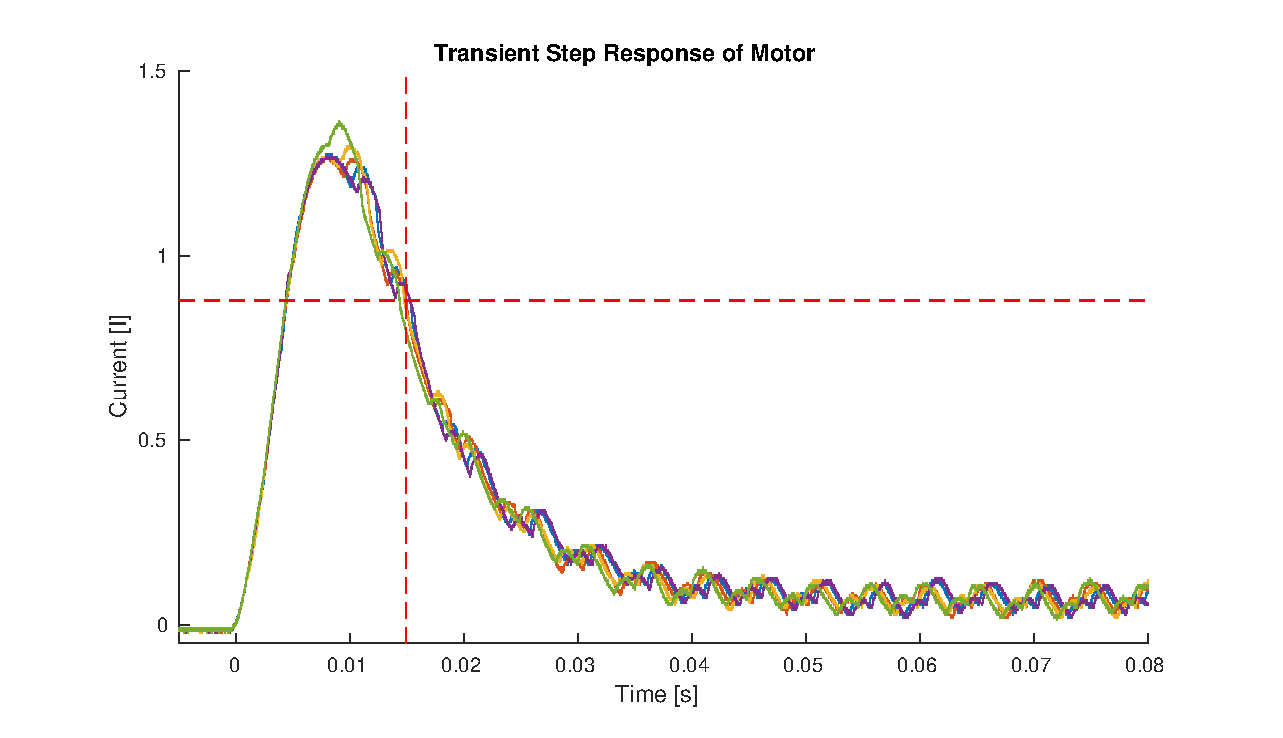
\includegraphics[width=\linewidth]{graphics/transient_response_inertia}
	\caption{Transient responses of the motor given a 7V step input. The horizontal line represent the value of $i_a(T)$ and the vertical line represents $T$.}
	\label{fig:inertia_trans_plot}
\end{figure}

With a step input of 7V and using the measured parameters, with the least deviation, for $K_{fm}$,$R_a$ and $K_m$ the mean value of $i_a(T)$ was calculated to be 0.88 I. 
The mean value of $T$ was then found to be 0.015 s and lastly the mean value of $J_r$, with a step input of 7V, was found to be $6.54 \cdot 10^{-6} \cdot kg \cdot m^2$.

\par
The mean value of $J_r$ from all the experiments with varying step input value was found to be $ 6.06 \cdot 10^{-6} \cdot kg \cdot m^2$ which is $45.4\%$ higher than the value given in the datasheet. 

\subsection{Comparison - Conclusion}
Throughout this section the experiments used to determine the various parameters of the Pittman 9324 have been presented.
Table~\ref{tab:compare} contains an overview and comparison with values given in the datasheet and those determined by experimentation.
As mentioned in section~\ref{sec:armature}, the armature resistance $R_a$ is quite high compared to the value given in the datasheet.
However, two methods have yielded approximately the same result which leads to the conclusion that either:
\begin{enumerate}
	\item The armature resistance is $\sim25$\% out of specification. 
	Although no tolerances are given in the datasheet this is highly unlikely.
	\item Either one of the instruments used for the measurements (2x Keysight 34410A) may be in need of calibration. 
	No evidence has been seen that this would be the case.
\end{enumerate}
At this time, no reasonable explanation for this deviation has been found.

\par
The voltage constant $K_e$ found in section~\ref{sec:voltconstat} is significantly closer to the given value and is easily acceptable.

\par
Similarly, when accounting for the coulomb friction and static friction the viscous damping factor found in section~\ref{sec:viscous} is very close to the given value.

\par
Two methods were used in section~\ref{sec:incuctance} for finding the inductance of the motor.
Method I showed a value close to given value, but the found values seemed to depend on the chosen size of $R_e$ although no explanation to this was found. 
Method II showed a dependency of frequency and the mean value of inductance between 25kHz and 35kHz was found to be quite large compared to the datasheet.

\par
In section~\ref{sec:inertia} the inertia of the motor was found using the measured transient response of the system.
The found value deviates from the datasheet value quite a lot. 
This could be partly due to the use of measured parameters in the calculation.

\begin{table}
	\centering
	\begin{tabular}{|l|c|c|c|}
		\hline
		Parameter & Datasheet & Experiment & \%'age\\
		\hline
		$R_a$ [$\Omega$] (M1/M2) & 2.96 & 3.647/3.715 & 23.21\%/25.51\%\\
		$K_e$ [$V\cdot\frac{S}{Rad}$]& 0.0365 & 0.036 & 1.37\%\\
		$K_v$ [$Nm\cdot\frac{S}{Rad}$]& $2.6\cdot10^{-6}$ & $2.611\cdot10^{-6}$ & 0.42\%\\
		$L_a$ [$mH$] (M1/M2)& 2.51 & 2.6/2.1 & 3.59\% / 17.7\%\\
		$J_r$ [$kg\cdot m^2$]& $4.2\cdot10^{-6}$& $6.06 \cdot10^{-6}$ & 45.4\%\\
		\hline
	\end{tabular}
	\caption[Comparison of parameter values.]{Comparison between the parameter values of the Pittman 9324 given in the datasheet and the values found by experimentation. The final column shows the percentage-wise deviation between the two values.}
	\label{tab:compare}
\end{table}

\newpage
%!TEX root = ../main.tex
\section{Designing a controller}
\label{sec:controller}

\todo{PUT DOTS AT the end of figures' sentences}
\todo[inline]{A Simulink block diagram -Mikkel}
To control the speed of the DC motor a controller will have to be implemented to the system. A block diagram of the DC motor in figure~\ref{fig:dcmotormodel} is shown in figure~\ref{fig:dcblock}. From the block diagram the transfer function $P(s)$ of the motor can be derived as seen in equation~\ref{eq:fullplant}. $P(s)$ is rearranged to coincide with the form in equation~\ref{eq:simpleplant}. From the block diagram a transfer function $P(s)$ for the motor can be derived as seen in equation~\ref{eq:fullplant} on the form in equation~\ref{eq:simpleplant}.\todo{During pull, this paragraph was messed up. I fixed it, but all of you take a look at it just in case to see if it's ok.}

\begin{figure}[!h]
	\centering
	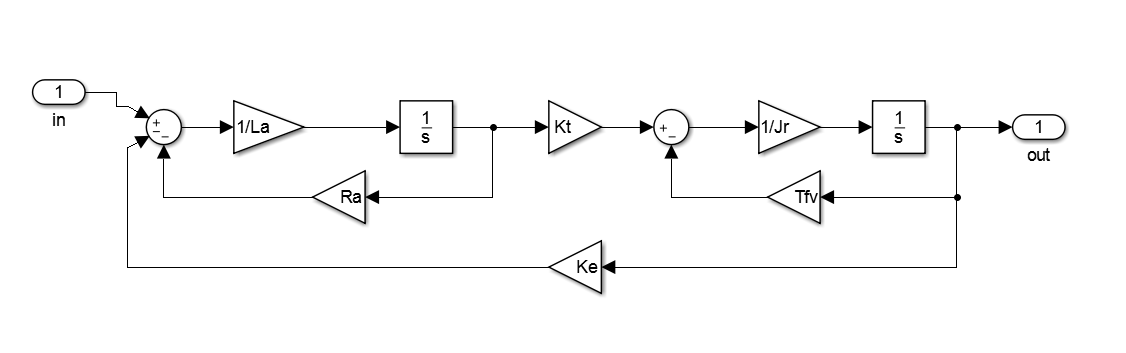
\includegraphics[width=1\linewidth]{graphics/dcblockdiagram}
	\caption{A block diagram of the full order DC motor.}
	\label{fig:dcblock}
\end{figure}


\begin{equation}
\label{eq:fullplant}
P(s) = \dfrac{\dfrac{K_m}{J_r L_a}}{s^2 + \dfrac{J_r R_a + L_a T_{fv}}{J_r L_a}s + \dfrac{R_a T_{fv} +K_m^2}{J_r L_a}}
\end{equation}

\begin{equation}
\label{eq:simpleplant}
P(s) = \dfrac{b_0}{s^2 + a_1 s + a_0}
\end{equation}


\subsection{PID controller}
 A commonly used controller is the PID controller~\cite{feedback}. 
 The name comes from its three adjustable parameters, the proportional gain $K_{P}$, integral gain $K_{I}$ and the derivative gain $K_{D}$. 
 The reason for its popularity is the wide range of operating conditions as well as being relatively easy to understand. 
 
 The controller is placed at the input of the motor, monitoring the output through a feedback. 
 The system is shown in figure~\ref{fig:pidcontrolsystem} where the plant is the DC motor. 
 The transfer function $H(s)$ of the system is shown in equation~\ref{eq:tfpidsystem} where $C(s)$ is the transfer function of the controller.

\begin{figure}[!h]
	\centering
	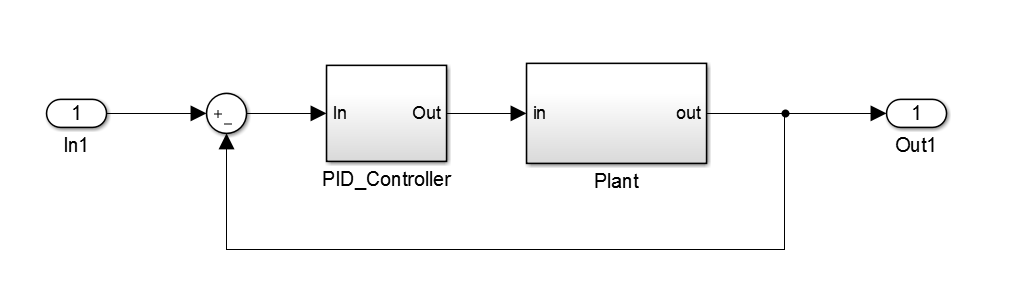
\includegraphics[width=.75\linewidth]{graphics/controlsystem}
	\caption{Block diagram of the PID control system. The plant represents the DC motor.}
	\label{fig:pidcontrolsystem}	
\end{figure}

\begin{equation}
\label{eq:tfpidsystem}
H(s) = \dfrac{C(s)P(s)}{1+C(s)P(s)}
\end{equation}

A block diagram for the PID controller can be seen in figure~\ref{fig:pidblock} and its transfer function in equation~\ref{eq:pid}.  

\begin{figure}[!h]
	\centering
	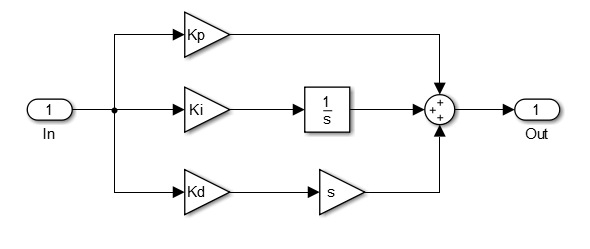
\includegraphics[width=.7\linewidth]{graphics/pidcontroller}
	\caption{Block diagram of the PID-controller}
	\label{fig:pidblock}
\end{figure}

\begin{equation}
\label{eq:pid}
C(s) = K_P + \dfrac{K_I}{s} +K_D s
\end{equation}

Inserting the transfer functions $C(s)$ and $P(S)$ into the transfer function $H(s)$ and rearranging it, $H(s)$ becomes equation~\ref{eq:pidfulltf}. On this form, the denominator describes the poles of the system. The denominator is the system's characteristic equation.

\begin{equation}
\label{eq:pidfulltf}
H(s) = \dfrac{b_0 (K_D s^2 + K_P s K_I)}{s^3 + (a_1 + b_0 K_D)s^2 (a_0 + b_0 K_P)s + b_0 K_I }
\end{equation}


\subsection{IPD controller}
An equivalent setup to the PID controller is the IPD controller, which does not introduce zeros to the system. It still uses the same gains, proportional, integral and derivative.

\begin{figure}[!h]
	\centering
	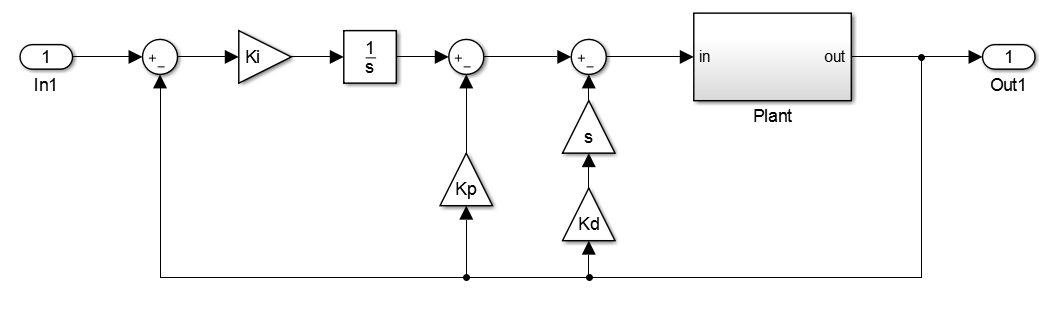
\includegraphics[width=1\linewidth]{graphics/ipdcontroller}
	\caption{Block diagram of the IPD control setup}
	\label{fig:ipdcontrolsystem}	
\end{figure}

The transfer function of the IPD controller system becomes as seen in equation~\ref{eq:tfipdsystem}. The transfer functions $P(s)$ and $C(s)$ are the same as in equation~\ref{eq:tfpidsystem}. It is noticed that the transfer function indeed introduces no zeros to the system.

\begin{equation}
\label{eq:tfipdsystem}
H(s) = \dfrac{\dfrac{K_I}{s} P(s)}{1+C(s)P(s)}
\end{equation}

With insertion and rearranging, the transfer function $H(s)$ takes the form of equation~\ref{eq:ipdfulltf}. Now it can be seen that indeed the IPD controller does not introduce any zeros to the system and the characteristic equation is the same as the one for the PID controller. Thus the same controller gains can be used in both cases.

\begin{equation}
\label{eq:ipdfulltf}
H(s) = \dfrac{b_0 K_I}{s^3 + (a_1 + b_0 K_D)s^2 (a_0 + b_0 K_P)s + b_0 K_I }
\end{equation}

\subsection{Noise Filtering}

The derivative part of the PID controller will try to reduce every sudden change in the system. This is what helps the system stop oscillating. However, when noise is introduced into the system, the derivative term acts on the fast, sudden change and can destabilize the system. In other words, the derivative term can and will increase the noise. For this reason a low pass filter is needed on the derivative path. This is done with changing $s$ on the derivative gain to $N/(s + N)$ where $N$ is $1/T_f$ and $T_f$ is the filter time constant and N is the cut off frequency. The block diagram for the controllers then become as seen in figures~\ref{fig:pidfilter} and~\ref{fig:ipdfilter} respectively.

\begin{figure}[!h]
	\centering
	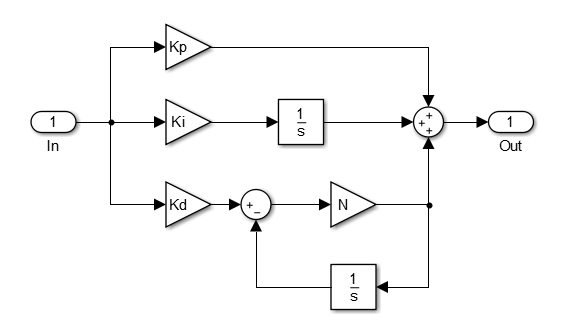
\includegraphics[width=.7\linewidth]{graphics/pidwfilter}
	\caption{Block diagram of the PID controller with filter}
	\label{fig:pidfilter}
\end{figure}

\begin{figure}[!h]
	\centering
	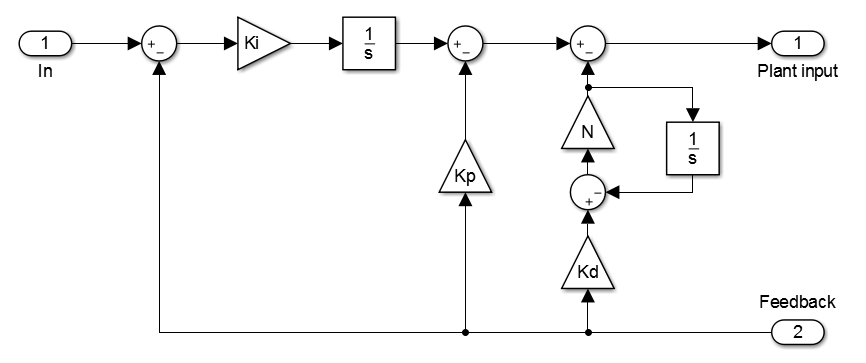
\includegraphics[width=.9\linewidth]{graphics/ipdwfilter}
	\caption{Block diagram of the IPD controller with filter}
	\label{fig:ipdfilter}
\end{figure}


\subsection{Anti-Windup Design}
\todo[inline]{Maybe we should tell that saturation is the source of the nonlinear region. And explain why antiwindup is needed. I think we also should write something else than "smoother behavior" as it is not very much in engineering terms-Mikkel}
During the function of the controller, there is a possibility that it will operate in a nonlinear region where increasing the control signal has no effect on the system output. This introduces time delay to the response of the system, thus reducing its overall performance. This behaviour can be counteracted using an anti-windup strategy such as the one in figure~\ref{fig:ipdantiwindupstrategy}.

\begin{figure}[!h]
	\centering
	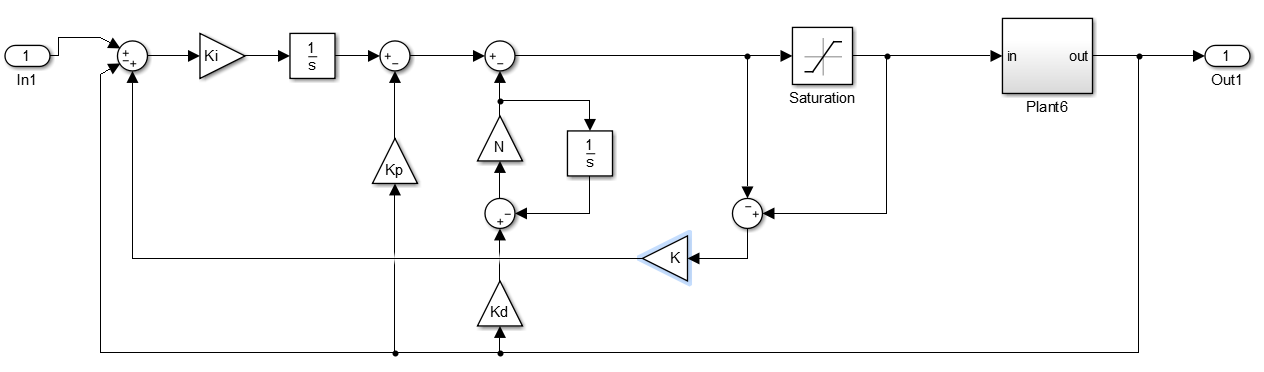
\includegraphics[width=1\linewidth]{graphics/ipdwindupdesign}
	\caption{Block diagram of the IPD controller with anti-windup design}
	\label{fig:ipdantiwindupstrategy}
\end{figure}

As figure~\ref{fig:antiwindupresponses} shows, using this strategy introduces smoother behaviour into the system. The gain $K$ is the one that determines that behaviour and can be chosen doing experiments using trial and error. An interesting observation is that the value of $K$ for the PID controller is quite different from the one for the IPD controller. Specifically, a suitable value for PID is $K=10$, while for IPD is $K=10000$. That conclusion has been reached through experiments, and the results can be seen in figure~\ref{fig:pidwindupvaluecomp}.

One major disadvantage of implementing such a strategy is that the settling time suffers for low values. This phenomena can be seen in figure~\ref{fig:antiwindupresponses} where the desired settling time of $T_s$ = 0.01 is giving an error of approximately 55\%.
\begin{figure}
	\centering
	\begin{subfigure}[b]{0.45\textwidth}
		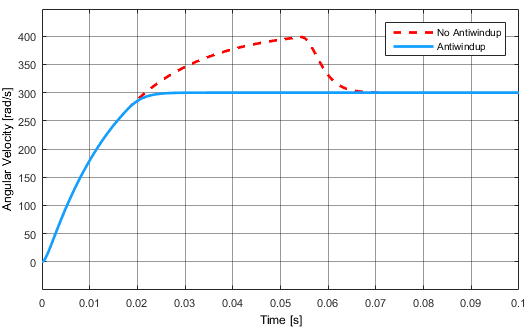
\includegraphics[width=\textwidth]{graphics/pidwindupresponse}
		\caption{PID controller.}
		\label{fig:pidwindupresponse}
	\end{subfigure}
	~ %add desired spacing between images, e. g. ~, \quad, \qquad, \hfill etc. 
	%(or a blank line to force the subfigure onto a new line)
	\begin{subfigure}[b]{0.45\textwidth}
		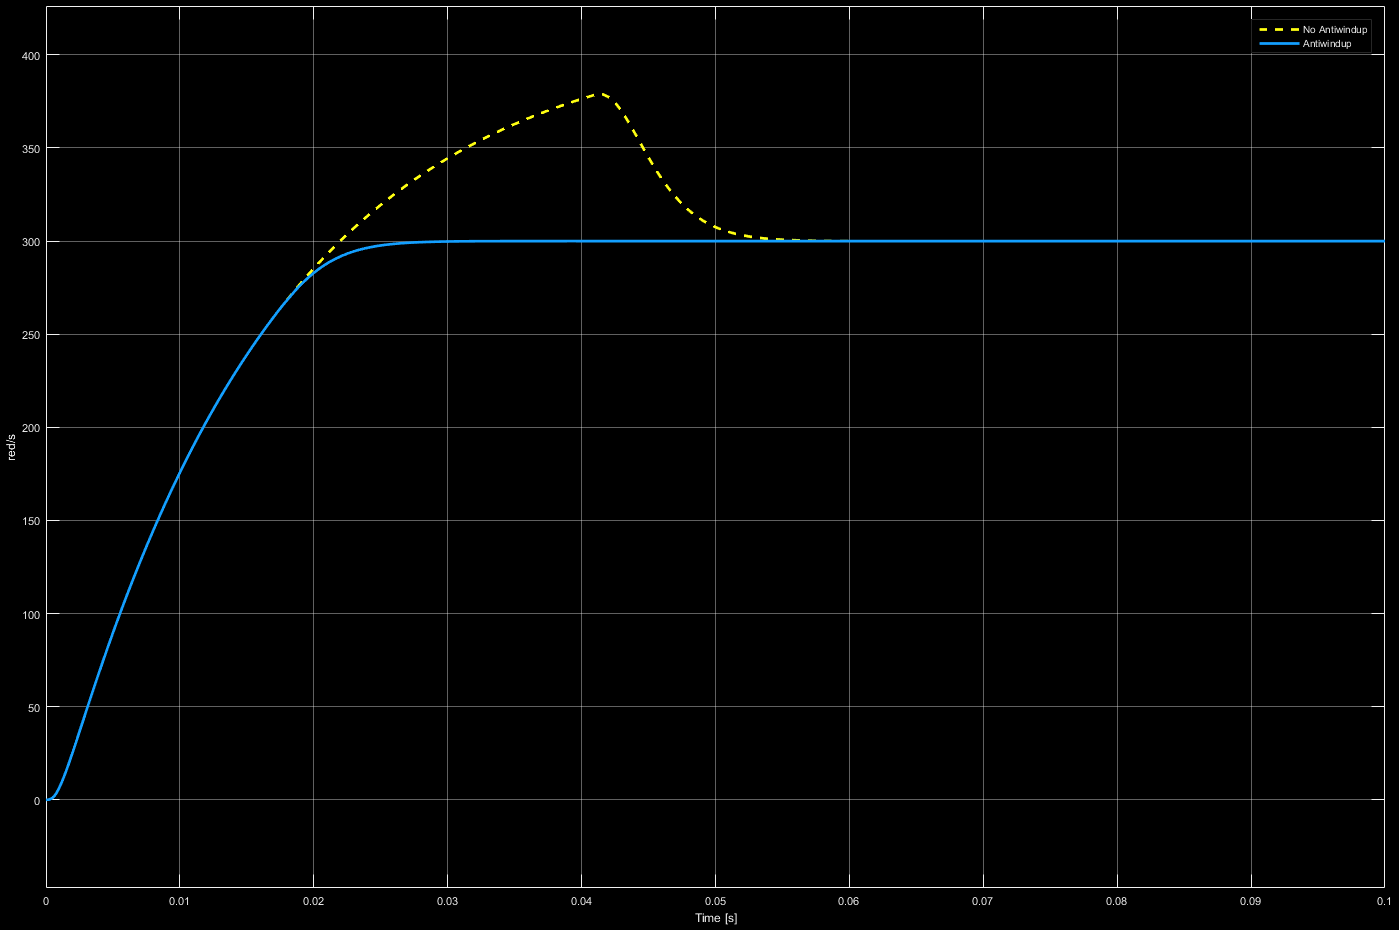
\includegraphics[width=\textwidth]{graphics/ipdwindupresponse}
		\caption{IPD controller.}
		\label{fig:ipdwindupresponse}
	\end{subfigure}
	\caption{Responses of controllers without and with anti-windup design.}\label{fig:antiwindupresponses}
\end{figure}

\todo[inline]{Not sure I understand this graph. We should discuss tomorrow -Mikkel}
\todo[inline]{Maybe we need to show a graph of what the antiwindup is really doing?-Mikkel}
\begin{figure}[!h]
	\centering
	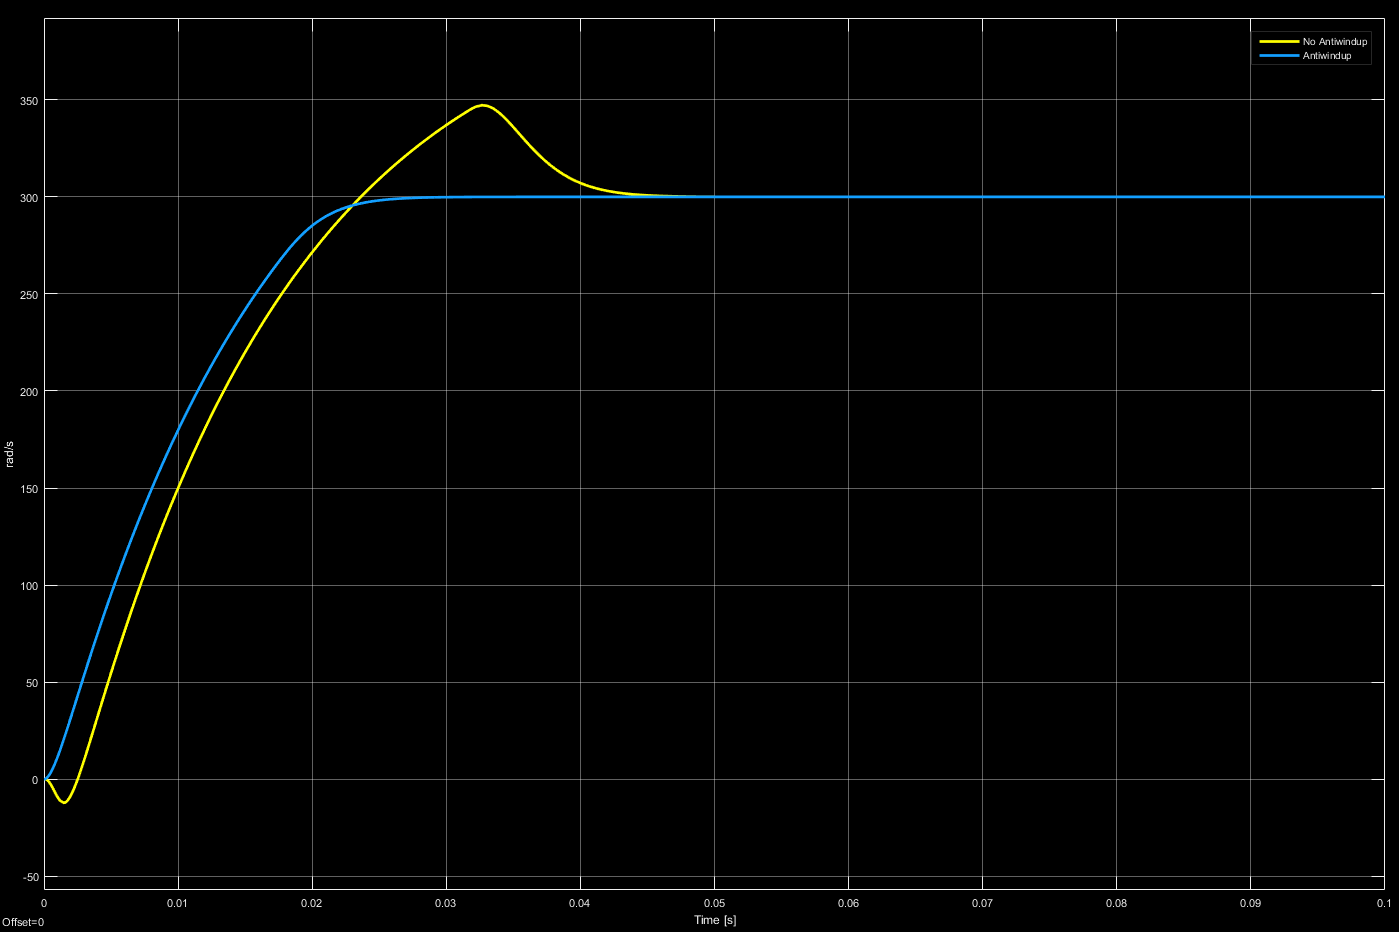
\includegraphics[width=.6\linewidth]{graphics/pidwindupvaluecomp}
	\caption{PID behaviour with different anti-windup gain. The higher gain being 10000 while the lower is 10.}
	\label{fig:pidwindupvaluecomp}
\end{figure}

\subsection{Controller Gain Design}
The controller gains are then to be designed. To achieve that the settling time method is introduced.


\subsubsection{Settling Time Formula}

The equation~\ref{eq:settling} is used for the system's desired response to enter the 5$\%$ error band within a specified settling time of $T_s$ and $n$ being the order of the controller.
\begin{equation}
\centering
\label{eq:settling}
\alpha = \dfrac{1.5(1 + n)}{T_s}
\end{equation}

\begin{table}[!h]
	\caption{ Coefficients of
		closed loop differential
		equation based on settling
		time formula~\cite{feedback}}
	\centering
	\begin{tabular}{|c|c|c|c|}
		\hline
		n & 2 & 3 & 4\\
		\hline
		$d_0$ & $\alpha^2$ & $\alpha^3$ & $\alpha^4$\\ 
		$d_1$ & $2\alpha$ & $3\alpha^2$ & $4\alpha^3$\\
		$d_2$ & - & $3\alpha$ & $6\alpha^2$\\
		$d_0$ & - & - & $4\alpha$\\
		\hline	
		
	\end{tabular}
	\label{table:coefsettlingtime}
\end{table}


\subsubsection{Full Order Systems}

As the equations~\ref{eq:pidfulltf} and~\ref{eq:ipdfulltf} show, their denominator is in the standard form of equation~\ref{eq:stdchararacteristic}. To calculate the controller gains the characteristic equation is compared to the coefficients in table~\ref{table:coefsettlingtime} where the order of the system in this case is $n=3$. The gain equations for $K_I, K_P$ and $K_D$ can be seen in equations~\ref{eq:pidki},~\ref{eq:pidkp} and~\ref{eq:pidkd} respectively. 


\begin{equation}
\centering
\label{eq:stdchararacteristic}
s^n + d_{n-1}s^{n-1} + \cdots + d_1 s + d_0 
\end{equation}

\begin{align}
\label{eq:pidki}
d_0 &= b_0 K_I = \alpha^3
\\
\label{eq:pidkp}
d_1 &= a_0 + b_0 K_P = 3\alpha^2
\\
\label{eq:pidkd}
d_2 &= a_1 + b_0 K_D = 3\alpha
\end{align}

Solving the above equations using the parameters and $T_s$ = 10~ms, the gains receive the values:
\begin{align*}
K_I &= 62.3855
\\
K_P &= 0.2752
\\
K_D &= 1.7910\cdot10^{-4}
\end{align*}

\todo[inline]{What is the settling time in the first example and why do we calculate two times? -Mikkel}
And again for a settling time $T_s$ = 100~ms

\begin{align*}
K_I &= 0.0945
\\
K_P &= -0.0315
\\
K_D &= -5.3532\cdot10^{-4}
\end{align*}


\subsubsection{Reduced Order Systems}
\todo[inline]{We should tell why we can reduce the order. Maybe a pole zero plot -Mikkel}
In the case of a reduced order system, the controller derivative's gain is equal to zero and the inductance of the motor $L_a$ is not taken into account during the calculations. The reduced transfer function takes the form of equation~\ref{eq:pireducedtf}.

\begin{equation}
\label{eq:pireducedtf}
H(s) = \dfrac{b_0(K_Ps + K_I)}{s^2 + (a_0 + b_0 K_P)s + b_0 K_I }
\end{equation}

Matching the characteristic equation with the standard form and looking at the coefficients in table~\ref{table:coefsettlingtime}, the equations for the controller gains, $K_i$ and $K_p$ become as seen in equations~\ref{eq:piki} and~\ref{eq:pikp} respectively.

\begin{align}
\label{eq:piki}
d_0 &= b_0 K_I = \alpha^2
\\
\label{eq:pikp}
d_1 &= a_0 + b_0 K_P = 2\alpha
\end{align}

Similarly, using the parameters and $T_s=10ms$, the gains in this case are:

\begin{align*}
K_I &= 221
\\
K_P &= 0.7
\end{align*}
 
 and again for the settling time of $T_s$ = 100ms:
 
 \begin{align*}
 K_I &= 2.2101
 \\
 K_P &= 0.0374
 \end{align*}
 
\newpage
%!TEX root = ../main.tex
\section{Simulations}
Before the controllers can be tested on the real system a simulation must be done. The controllers that have been chosen are the IPD and PI, where PI is the PID controller with $K_D$ set to 0. Speed control is simulated at two different angular velocities, \todo{To different step signals ? - Mikkel}200~rad/s and~125 rad/s. To prevent the saturation limit to be reached, the settling time is set to 0.1~ms.\todo{why settling time 0.1 and not 0.01}
\todo[inline]{Why are these choosen? -Mikkel}
\begin{figure}[h!]
	\centering
	\begin{subfigure}[b]{0.45\textwidth}
		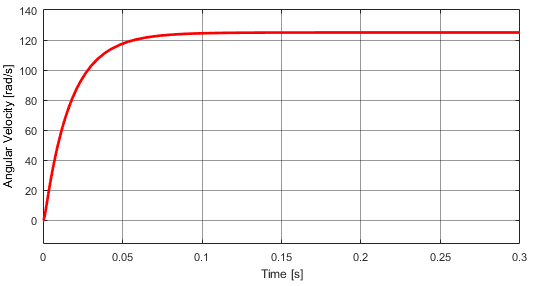
\includegraphics[width=\textwidth]{graphics/PI_single125}
		\caption{PI Speed control at 125 rad/s.}
		\label{fig:pisingle125}
	\end{subfigure}
	~ %add desired spacing between images, e. g. ~, \quad, \qquad, \hfill etc. 
	%(or a blank line to force the subfigure onto a new line)
	\begin{subfigure}[b]{0.45\textwidth}
		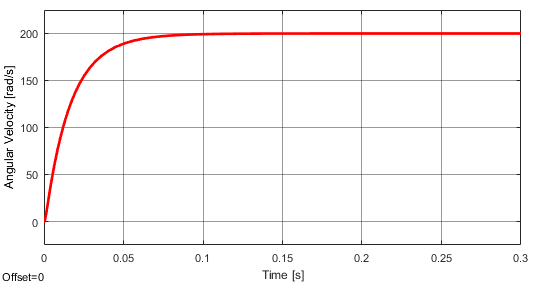
\includegraphics[width=\textwidth]{graphics/PI_single200}
		\caption{PI Speed control at 200 rad/s.}
		\label{fig:pisingle200}
	\end{subfigure}
	\caption{The PI controller at two different angular velocities. It is noticed that the desired settling time is reached in both cases.}\label{fig:pisingle}
\end{figure}






\begin{figure}[h!]
	\centering
	\begin{subfigure}[b]{0.45\textwidth}
		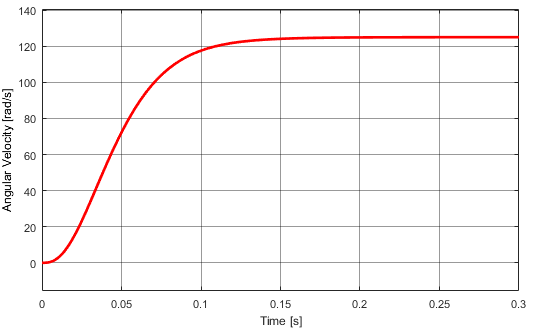
\includegraphics[width=\textwidth]{graphics/IPD_single125}
		\caption{IPD Speed control at 125 rad/s.}
		\label{fig:ipdsingle125}
	\end{subfigure}
	~ %add desired spacing between images, e. g. ~, \quad, \qquad, \hfill etc. 
	%(or a blank line to force the subfigure onto a new line)
	\begin{subfigure}[b]{0.45\textwidth}
		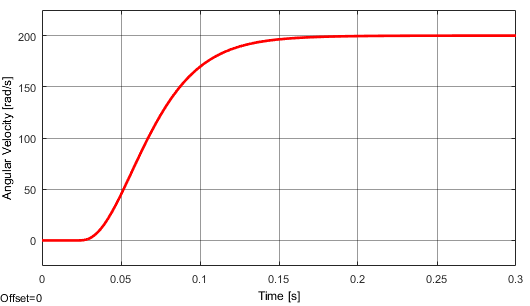
\includegraphics[width=\textwidth]{graphics/IPD_single200}
		\caption{IPD Speed control at 200 rad/s.}
		\label{fig:ipdsingle200}
	\end{subfigure}
	\caption{The IPD controller at two different angular velocities. A delay is introduced. The desired settling time is reached from when the controller responses.}\label{fig:ipdsingle}
\end{figure}
\todo{The sentence may need to be expressed again? "The desired...the controller}

\todo[inline][We should be able to find out where the delay comes from? - Mikkel]
The simulation confirms that the controllers behave similar for both simulated angular velocities as seen in figures~\ref{fig:pisingle} and~\ref{fig:ipdsingle}. Both the PI and IPD achieve to settle within the specified settling time. However, an unexplained delay is introduced in the beginning of the IPD controller response. That delay does not affect the system response in other way than offsetting it.

\begin{figure}[h!]
	\centering
	\begin{subfigure}[b]{0.45\textwidth}
		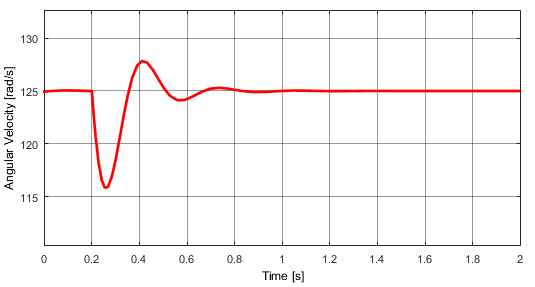
\includegraphics[width=\textwidth]{graphics/PI_load125}
		\caption{PI Speed control at 125 rad/s.}
		\label{fig:piload125}
	\end{subfigure}
	~ %add desired spacing between images, e. g. ~, \quad, \qquad, \hfill etc. 
	%(or a blank line to force the subfigure onto a new line)
	\begin{subfigure}[b]{0.45\textwidth}
		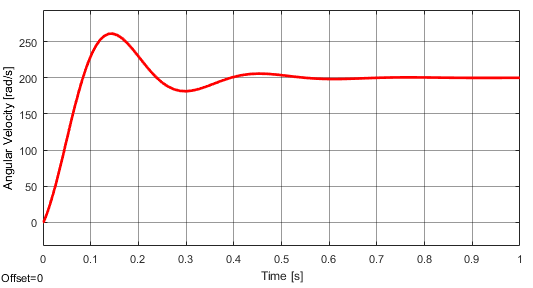
\includegraphics[width=\textwidth]{graphics/PI_load200}
		\caption{PI Speed control at 200 rad/s.}
		\label{fig:piload200}
	\end{subfigure}
	\caption{The PI controller at two different angular velocities with added load. Desired settling time is not reached. Instead, it introduces an overshoot and does not become stable until it is close to 1s.}
	\label{fig:piload}
\end{figure}

\begin{figure}[h!]
	\centering
	\begin{subfigure}[b]{0.45\textwidth}
		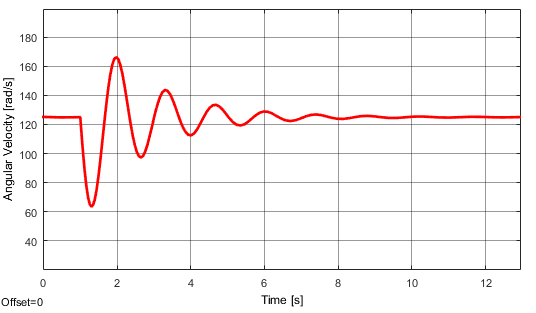
\includegraphics[width=\textwidth]{graphics/IPD_load125}
		\caption{IPD Speed control at 125 rad/s.}
		\label{fig:ipdload125}
	\end{subfigure}
	~ %add desired spacing between images, e. g. ~, \quad, \qquad, \hfill etc. 
	%(or a blank line to force the subfigure onto a new line)
	\begin{subfigure}[b]{0.45\textwidth}
		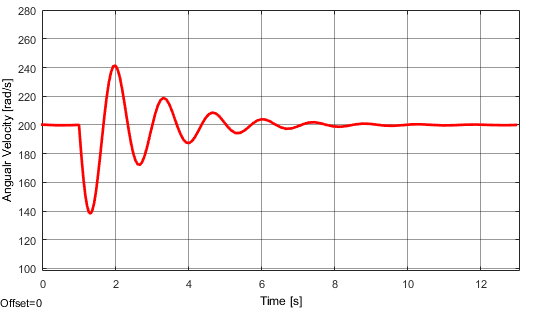
\includegraphics[width=\textwidth]{graphics/IPD_load200}
		\caption{IPD Speed control at 200 rad/s.}
		\label{fig:ipdload200}
	\end{subfigure}
	\caption{The IPD controller at two different angular velocities with added load. The desired settling time is far from being reached. The system becomes stable at around 13s.}
	\label{fig:ipdload}
\end{figure}
\todo{5.4 figures is referring to IPD controller, right? PI was written here.}

When the system has reached the stable output a load step is introduced.
When the load step is added, the IPD controller seems to have a hard time to settle, as it can be shown from figure~\ref{fig:ipdload}. The systems does not reach the stable condition until after 13s. This result could have been estimated thus the controllers were designed with only a single motor in mind. Added load changes the system behaviour and should be controlled with different controller gains.\todo{Catalin: I don't understand the sentence "This result...mind"}

\newpage
%!TEX root = ../main.tex
\clearpage
\section{Performance}
This section describes the performance of the controllers created in section~\ref{sec:controller}.
The controllers will be applied to both the real and the simulated system in order to compare the results.

\subsection{PI Controller}
The block diagram of this controller can be seen in figure~\ref{fig:pidcontroller}, although $K_D$ is set to zero in the PI controller.
Two tests are conducted for the PI controller, a load step and a velocity step.

\begin{figure}[!h]
	\centering
	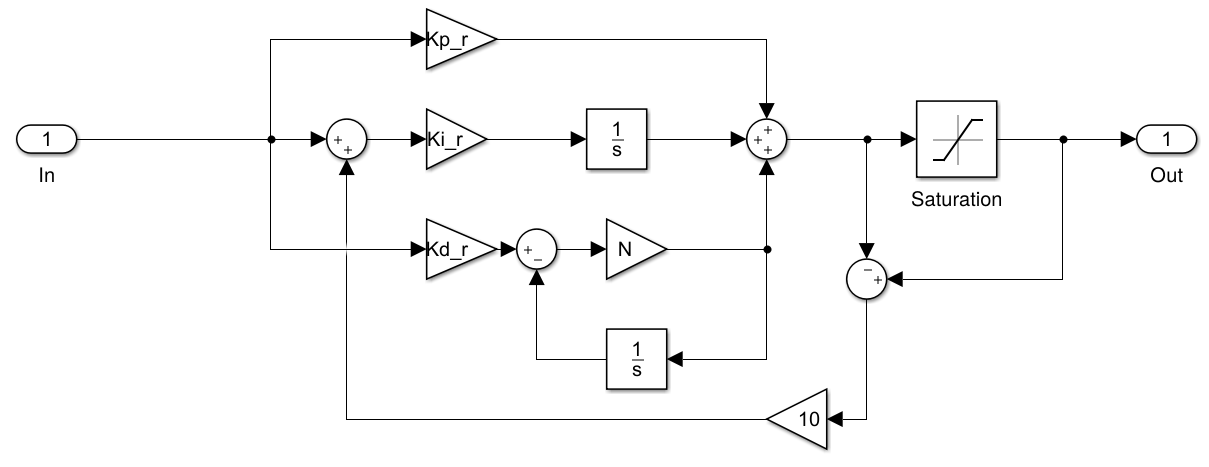
\includegraphics[width=.75\linewidth]{graphics/pid_controller}
	\caption{The implementation of the PID controller used with the dSpace system.}
	\label{fig:pidcontroller}
\end{figure}

\paragraph{Velocity Step:}~\\
A velocity step response was applied to the controller of values $\omega =$ 200, 250 and 400 $\frac{Rad}{S}$.
Note that at $\omega=400$ the controller was saturated significantly throughout the rise-time of the signal.
The result of these test can be seen on figure~\ref{fig:step}.
As it is expected when introducing an integral part to a controller, there is no appreciable steady-state error in either of the three cases.
There is, however, a ripple present on every test, most notably being at $\omega = 400$.
This is likely due to mechanical imperfections in the motor assembly.
Comparing the responses of the real and the simulated system in figures~\ref{fig:step200} and~\ref{fig:step200simulated}, respectively, although the real system has some overshoot that is not present in the simulation, the settling time is similar at $\approx50$ ms.

\begin{figure}[!h]
	\begin{subfigure}[t]{.49\linewidth}
		\centering
		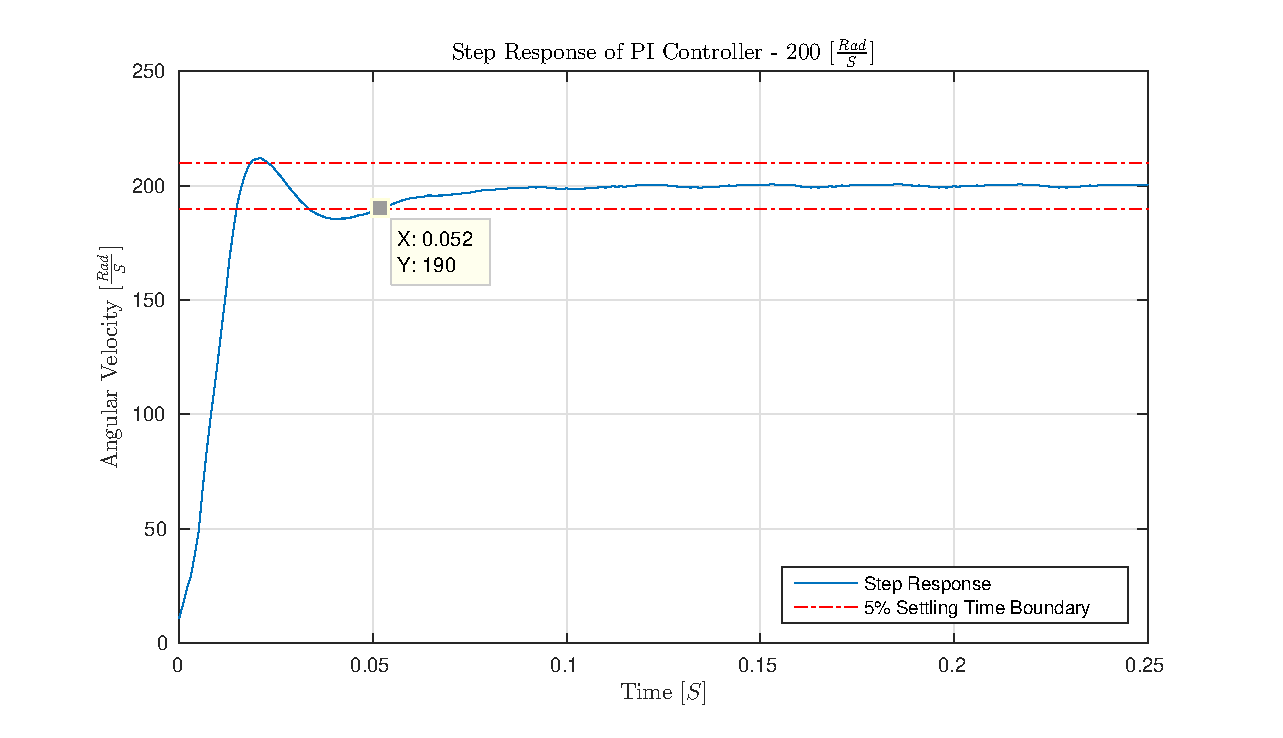
\includegraphics[width=\textwidth]{graphics/step_200_pi_real}
		\caption{Reference Step: $200 \frac{Rad}{S}$.}
		\label{fig:step200}
	\end{subfigure}
	\begin{subfigure}[t]{.49\linewidth}
		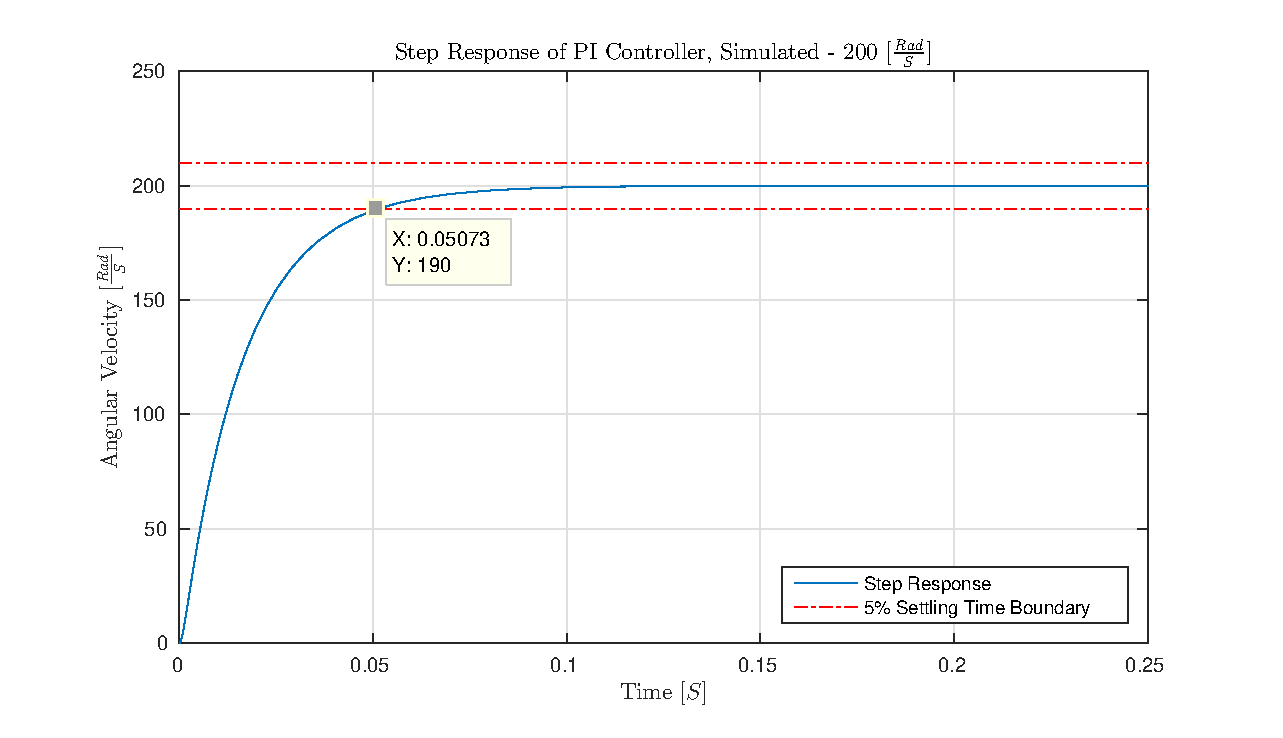
\includegraphics[width=\textwidth]{graphics/step_200_pi_simulated}
		\caption{Reference Step: $200 \frac{Rad}{S}$.}
		\label{fig:step200simulated}
	\end{subfigure}\\
	\centering
	\begin{subfigure}[t]{.49\linewidth}
		\centering
		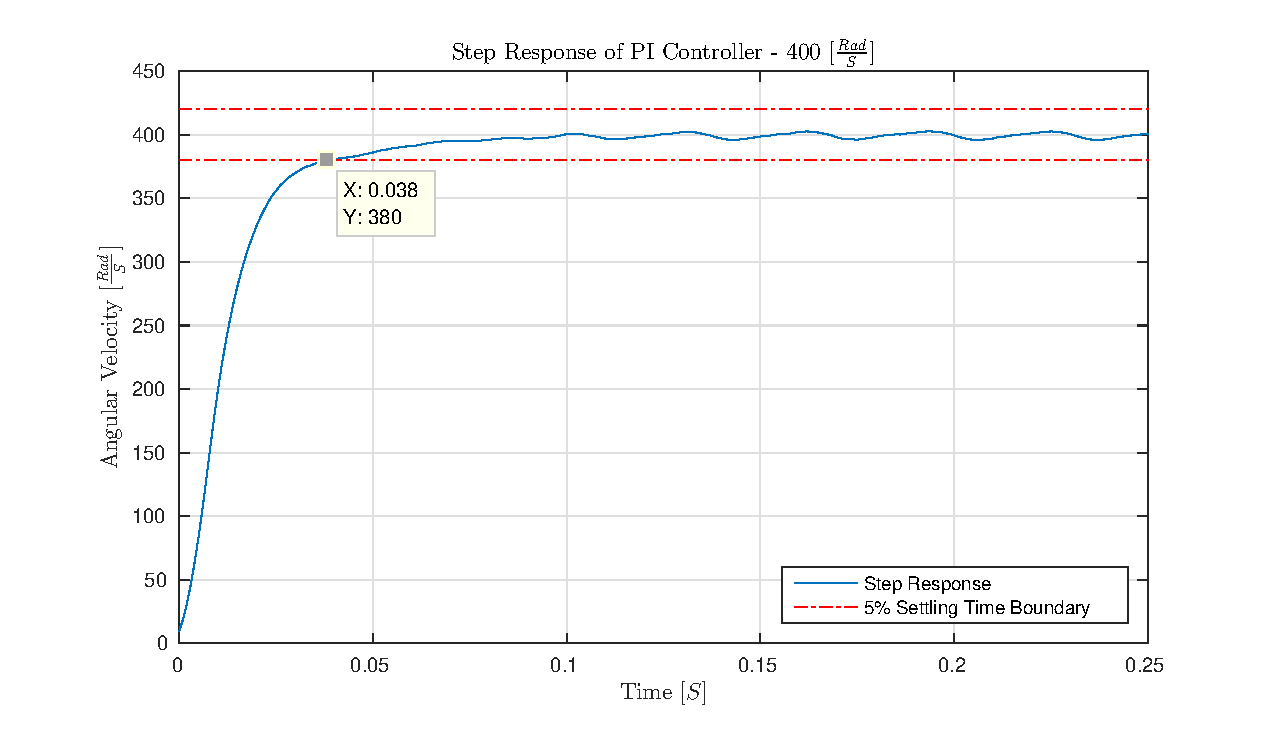
\includegraphics[width=\textwidth]{graphics/step_400_pi}
		\caption{Reference Step: $400 \frac{Rad}{S}$.}
		\label{fig:step400}
	\end{subfigure}
	\caption[Velocity step response of PI controller.]{Velocity step response of the PI controller. On each plot is marked the settling time of the response, $X$ in $[S]$.}
	\label{fig:step}
\end{figure}

Finally, the inertia was connected to the rotor of the motor and a reference step of $125\frac{Rad}{S}$ was applied.
As can be seen from~\ref{fig:stepinertia}, adding the extra inertia to the system greatly influences the performance of the controller.
The overshoot is greatly increased and the settling time lengthened by a factor of ten.
This is to be expected since the controller was designed without taking this inertia into account.
The responses in figures~\ref{fig:stepinertiareal} and~\ref{fig:stepinertiasimulated} are similar, but the overshoot on the real system is significantly higher than that on the simulated system.
This is likely due to the extra friction caused by bearings and other mechanical imperfections that are not modelled in the simulation.

\begin{figure}[!h]
	\begin{subfigure}[t]{.49\linewidth}
		\centering
		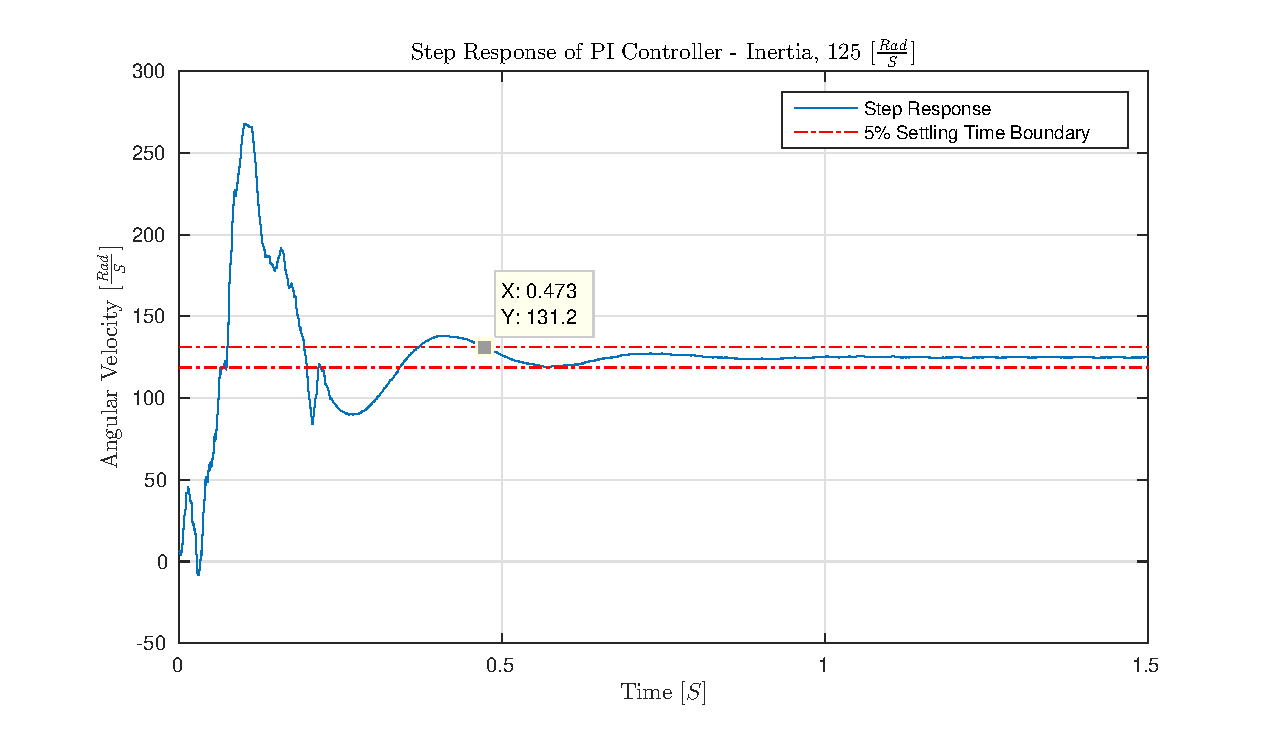
\includegraphics[width=\textwidth]{graphics/step_125_pi_inertia_real}
		\caption{Reference Step: $125 \frac{Rad}{S}$. Added inertia.}
		\label{fig:stepinertiareal}
	\end{subfigure}
	\begin{subfigure}[t]{.49\linewidth}
		\centering
		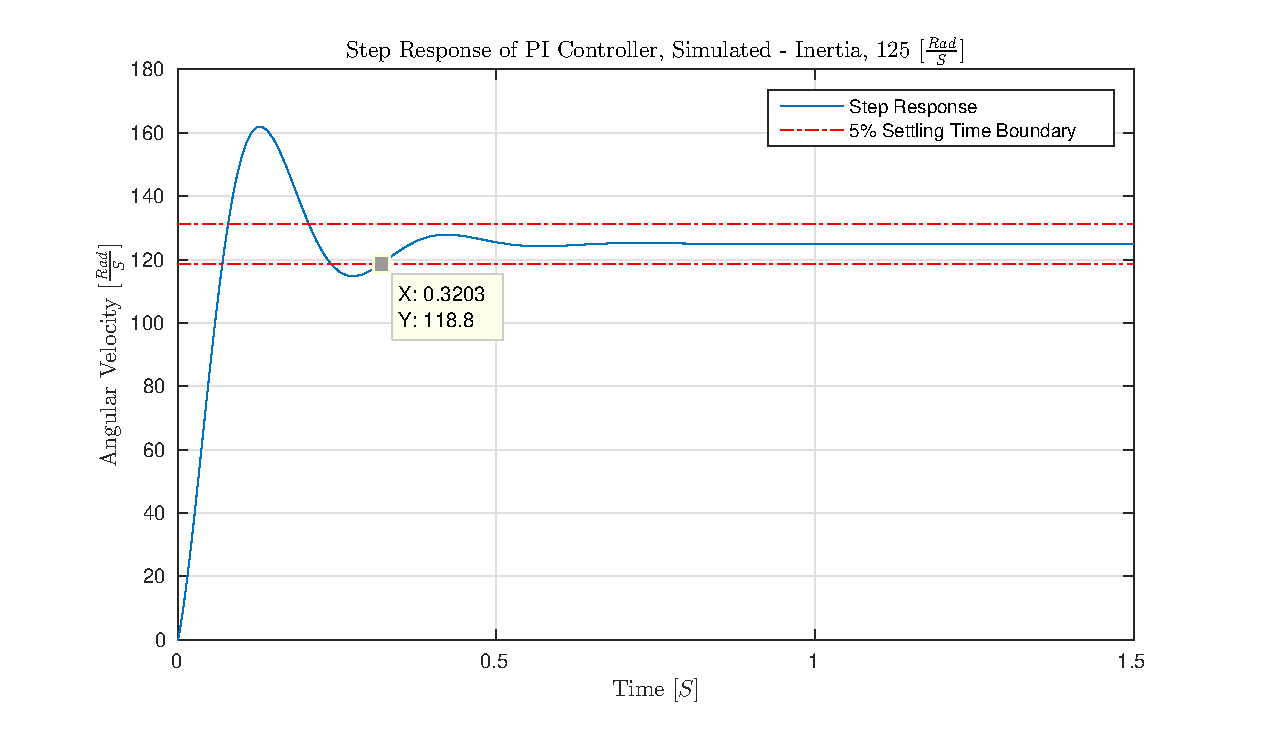
\includegraphics[width=\textwidth]{graphics/step_125_pi_inertia_simulated}
		\caption{Reference Step: $125 \frac{Rad}{S}$. Added inertia.}
		\label{fig:stepinertiasimulated}
	\end{subfigure}
	\caption[Velocity step response of PI controller with inertia.]{Velocity step response of the PI controller. On each plot the settling time of the response is marked, $X$ in $[S]$.}
	\label{fig:stepinertia}
\end{figure}

\paragraph{Load Step:}
The load step is performed by connecting both the inertia and the secondary motor to the rotor.
An electronic load is put in series with the terminals of the secondary motor.
This will allow for an easy way of limiting the current through the secondary motor, thus limiting the load generated.
The motor is now run at an angular velocity of $\omega=125\frac{Rad}{S}$.
Two loads were attempted: 0.4 and 0.5 $[A]$.
The results of this test can be seen in figure~\ref{fig:loadstep}.

\begin{figure}
	\begin{subfigure}[t]{.49\linewidth}
		\centering
		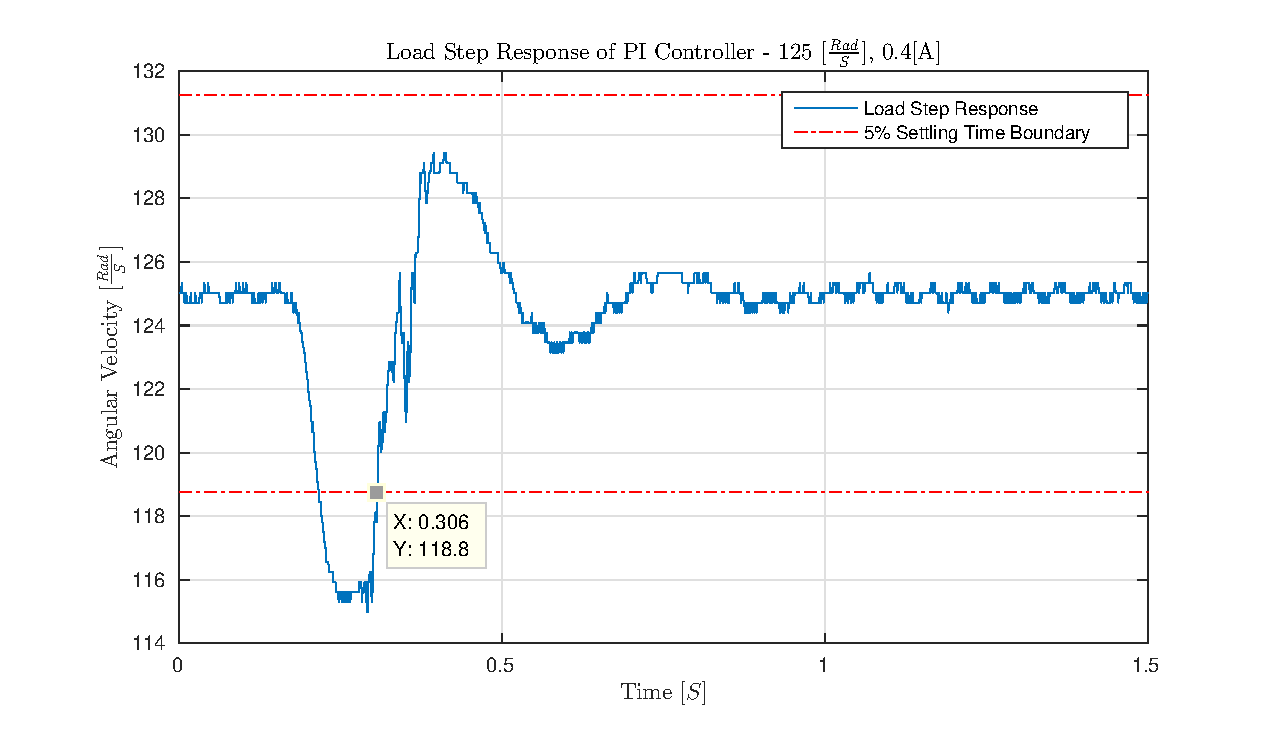
\includegraphics[width=\textwidth]{graphics/load_real}
		\caption{Reference Step: $0.4 [A]$.}
		\label{fig:loadstep04real}
	\end{subfigure}
	\begin{subfigure}[t]{.49\linewidth}
		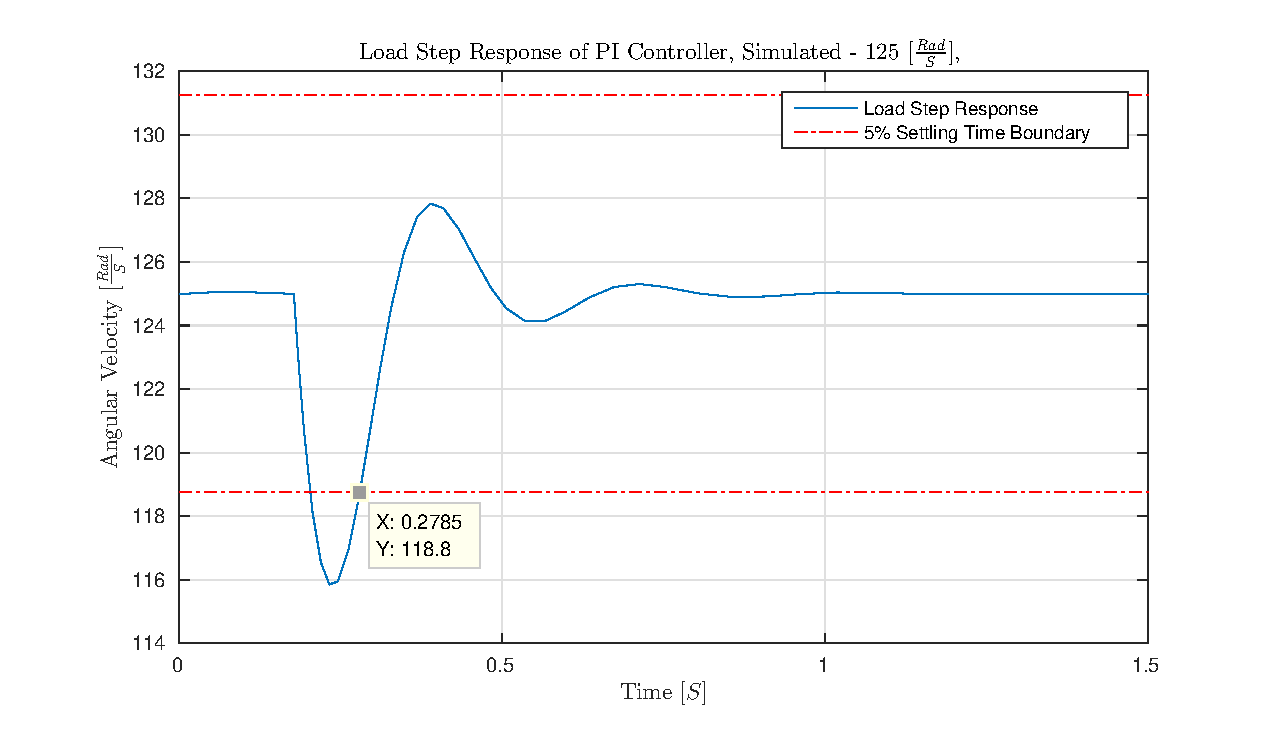
\includegraphics[width=\textwidth]{graphics/load_simulated}
		\caption{Reference Step: $0.4 [A]$.}
		\label{fig:loadstep04simulated}
	\end{subfigure}\\
	\centering
	\begin{subfigure}[t]{.49\linewidth}
		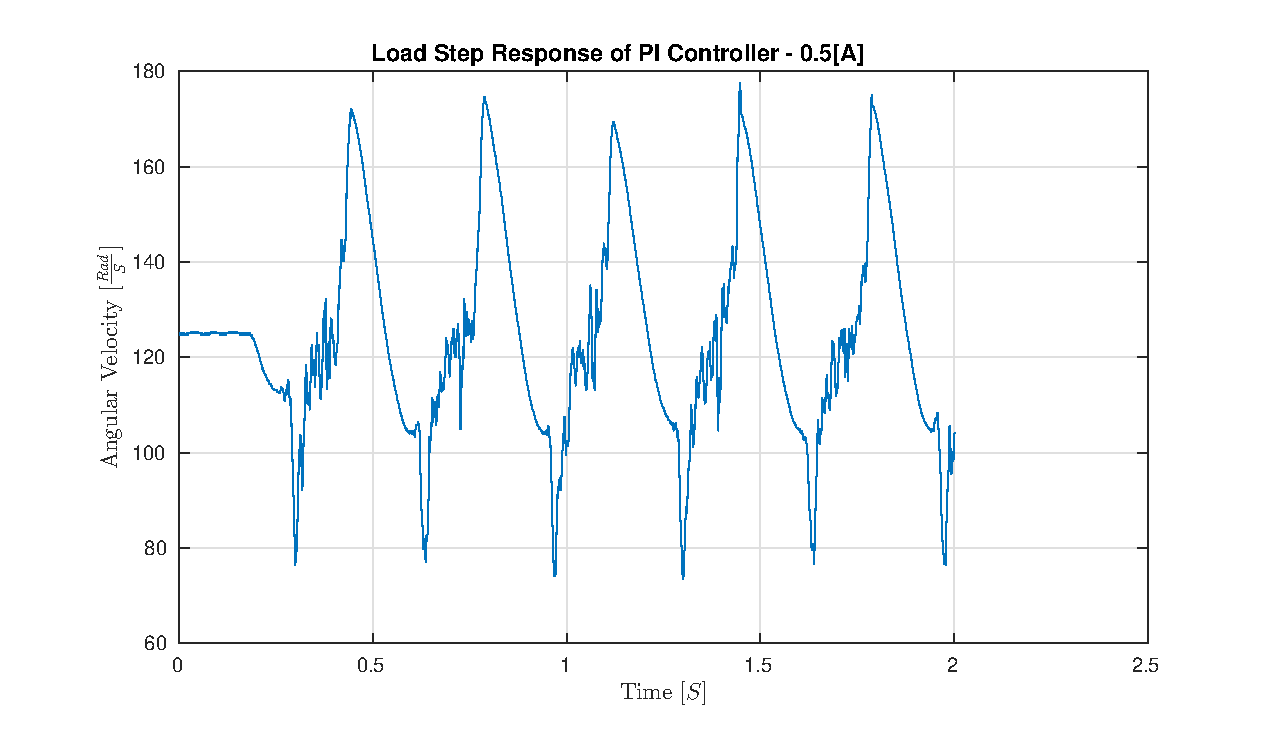
\includegraphics[width=\textwidth]{graphics/load_unstable}
		\caption{Reference Step: $0.5 [A]$.}
		\label{fig:}
	\end{subfigure}
	\caption[Load step response of PI controller]{Load step response of the PI controller. On each plot the settling time of the response is marked, $X$ in $[S]$.}
	\label{fig:loadstep}
\end{figure}

As can be seen, at the 0.5 $[A]$ reference step the controller becomes unstable.
The velocity continues to oscillate indefinitely.
Lowering the reference step slightly stabilises the response.
However due to the increased inertia on the system in this test the settling time is significant.
In this case, the real and simulated systems behaviours are very similar, both in settling time and the maximum and minimum peak values.
These can be seen in figures~\ref{fig:loadstep04real} and \ref{fig:loadstep04simulated} respectively.

\subsection{IPD Controller}
\begin{figure}[!h]
	\centering
	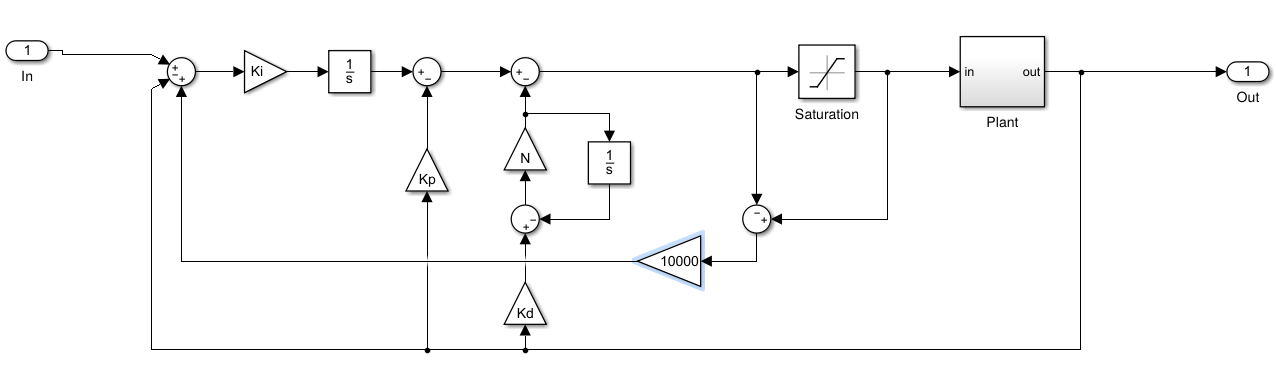
\includegraphics[width=.75\linewidth]{graphics/ipd_controller}
	\caption{The implementation of the IPD controller used with the dSpace system.}
	\label{fig:ipdcontroller}
\end{figure}

\todo{Rewrite for IPD - Thomas}
As with the PI controller, the block diagram of this controller can be seen in figure~\ref{fig:ipdcontroller}.
In fact, the only difference between these two controllers is the inclusion of the differential gain in the IPD controller.
This inclusion, however, gave rise to significant problems.
In order to have dSpace accepting the differential it was necessary to implement it as a low-pass filter.
By setting the cut-off frequency to a very high value this filtering should have no effect on the system.
This was found to not be the case. 
At values above $\approx$1000 the controller becomes unstable.
At these low values the filter still has a significant impact on the performance of the controller and it was not possible to obtain any sensible data on the performance of this controller.


\newpage
% !TeX root = ../main.tex
\section{Conclusion}

The report has gone through the steps required to design a control system for a DC motor and various conclusions have been drawn. The parameters from a motor's datasheet may not always coincide with the ones found by experimenting. In the case of the specific motor that the experiments were run, the inductance and the armature resistance are out of specification, 17.7\% and 25\% respectively, while the motor inertia deviates as well by an outstanding 45.4\%. 
\\

During the design of the PID and IPD controllers, one of the strategies that are implemented in order to make them more stable exhibits some differences in behaviour and efficiency, depending on the system. Specifically, the gain of the anti-windup design for the two controllers is completely different. A suitable gain for the PID is a value of 10, while for the IPD, 10000 is a far better value. On the other hand, the noise filtering is implemented with no differences to the various systems. Furthermore, the settling time suffers for very low values such as $T_s=0.01$ due to reaching the saturation of the system, which is counteracted by the anti-windup strategy, although not completely. Lastly, the characteristic equations of the two different controllers are the same, which contributes positively to the overall analysis.
\\

The simulations showed that for $T_s=0.1$ both controllers manage to reach their target within the specified settling time. 
However, that is not the case when a step load is introduced into the system. 
Adding a step load will result in approximately one second longer settling time, introducing an overshoot, but with no further difficulties. 
The IPD on the other hand takes more time to stabilize, requiring around $12S$. 
The real-world experiments showed some differences with the results of the simulations. 
During the velocity step experiment, the PI settles within the desired settling time with an overshoot not present in the simulation, while the load step behaviour was observed to be the same in both the experiment and the simulation. 
In the case of the IPD, satisfactory data could not be presented due to the implementation of the differential gain, which gave rise to major problems. Specifically, the cut-off frequency could not be set high enough in order to stabilize the system using dSpace.
\newpage
\begin{thebibliography}{11} %This number should be higher than the number of entries in the bibliography because reasons...
%	\bibitem{id}
%		Author(s) Last name, First name, Company/Organisation, Year. Full Title
	\bibitem{feedback}
		Dodds, Stephen J., University of East London, 2015. Feedback Control: Linear, Nonlinear and Robust Techniques and Design with Industrial Applications.
\end{thebibliography}

\end{document}

